\documentclass[a4paper]{article}
\usepackage[T1]{fontenc}			% \chapter package
\usepackage[english]{babel}
\usepackage[english]{isodate}  		% date format
\usepackage{graphicx}				% manage images
\usepackage{amsfonts}
\usepackage{booktabs}				% high quality tables
\usepackage{amsmath}				% math package
\usepackage{amssymb}				% another math package (e.g. \nexists)
\usepackage{bm}                     % bold math symbols
\usepackage{mathtools}				% emphasize equations
\usepackage{stmaryrd} 				% '\llbracket' and '\rrbracket'
\usepackage{amsthm}					% better theorems
\usepackage{enumitem}				% manage list
\usepackage{pifont}					% nice itemize
\usepackage{cancel}					% cancel math equations
\usepackage{caption}				% custom caption
\usepackage[]{mdframed}				% box text
\usepackage{multirow}				% more lines in a table
\usepackage{textcomp, gensymb}		% degree symbol
\usepackage[x11names]{xcolor}		% RGB color
\usepackage[many]{tcolorbox}		% colorful box
\usepackage{multicol}				% more rows in a table (used for the lists)
\usepackage{listings}
\usepackage{url}
\usepackage{qrcode}
\usepackage{fontawesome5}
\usepackage{ragged2e}
\usepackage{cite}                   % references
\usepackage{imakeidx}               % index
\makeindex[program=makeindex, columns=1,
           title=Index, 
           intoc,
           options={-s index-style.ist}]
\usepackage{fancyhdr}

%\pdfcompresslevel=0
%\pdfobjcompresslevel=0

\definecolor{codegreen}{rgb}{0,0.6,0}
\definecolor{codegray}{rgb}{0.5,0.5,0.5}
\definecolor{codepurple}{rgb}{0.58,0,0.82}
\definecolor{backcolour}{rgb}{0.95,0.95,0.92}
\lstdefinestyle{mystyle}{
    backgroundcolor=\color{backcolour},   
    commentstyle=\color{codegreen},
    keywordstyle=\color{magenta},
    numberstyle=\tiny\color{codegray},
    stringstyle=\color{codepurple},
    basicstyle=\ttfamily\footnotesize,
    breakatwhitespace=false,         
    breaklines=true,                 
    captionpos=b,                    
    keepspaces=true,                 
    numbers=left,                    
    numbersep=5pt,                  
    showspaces=false,                
    showstringspaces=false,
    showtabs=false,                  
    tabsize=2
}
\lstset{style=mystyle}


% thanks Mico: https://tex.stackexchange.com/a/60218/312896
\makeatletter
\renewcommand\paragraph{\@startsection{paragraph}{4}{\z@}%
            {-2.5ex\@plus -1ex \@minus -.25ex}%
            {1.25ex \@plus .25ex}%
            {\normalfont\normalsize\bfseries}}
\makeatother
\setcounter{secnumdepth}{4} % how many sectioning levels to assign numbers to
\setcounter{tocdepth}{4}    % how many sectioning levels to show in ToC


% draw a frame around given text
\newcommand{\framedtext}[1]{%
	\par%
	\noindent\fbox{%
		\parbox{\dimexpr\linewidth-2\fboxsep-2\fboxrule}{#1}%
	}%
}


% table of content links
\usepackage{xcolor}
\usepackage[linkcolor=black, citecolor=blue, urlcolor=cyan]{hyperref} % hypertexnames=false
\hypersetup{
	colorlinks=true
}


\newtheorem{theorem}{\textcolor{Red3}{\underline{Theorem}}}
\renewcommand{\qedsymbol}{QED}
\newcommand{\dquotes}[1]{``#1''}
\newcommand{\longline}{\noindent\rule{\textwidth}{0.4pt}}
\newcommand{\circledtext}[1]{\raisebox{.5pt}{\textcircled{\raisebox{-.9pt}{#1}}}}
\newcommand{\definition}[1]{\textcolor{Red3}{\textbf{#1}}\index{#1}}
\newcommand{\example}[1]{\textcolor{Green4}{\textbf{#1}}}
\newcommand{\highspace}{\vspace{1.2em}\noindent}


\begin{document}
    \newcounter{definition}[section]
    \newcounter{example}[section]
    \newcounter{exercise}[section]
    
    \newtcolorbox[use counter = definition]{definitionbox}{%
        breakable,
        enhanced,
        colback=red!5!white,
        colframe=red!75!black,
        fonttitle=\bfseries,
        title={Definition \thetcbcounter} %
    }

    \newtcolorbox[use counter = exercise]{exercisebox}[1][]{%
        breakable,
        enhanced,
        colback=Red3!5!white,
        colframe=Red3!75!black,
        fonttitle=\bfseries,
        title={Exercise \thetcbcounter#1} %
    }
    
    \newtcolorbox[use counter = example]{examplebox}[1][]{%
        breakable,
        enhanced,
        colback=Green4!5!white,
        colframe=Green4!75!black,
        fonttitle=\bfseries,
        title={Example \thetcbcounter#1} %
    }

    \newtcolorbox[]{deepeningbox}[1][]{%
        breakable,
        enhanced,
        colback=DarkOrange3!5!white,
        colframe=DarkOrange3!75!black,
        fonttitle=\bfseries,
        title={Deepening#1} %
    }

    %%%%%%%%%%%%%%%
    % Notes cover %
    %%%%%%%%%%%%%%%
    \author{260236}
\title{Parallel Computing - Notes - \version}
\date{\printdayoff\today}
\maketitle

    %%%%%%%%%%%
    % Preface %
    %%%%%%%%%%%
	\section*{Preface}

Every theory section in these notes has been taken from the sources:
\begin{itemize}
    \item Course slides.\cite{numerical-linear-algebra-polimi}
\end{itemize}
About:
\begin{itemize}
    \item[\faIcon{github}] \href{https://github.com/PoliMI-HPC-E-notes-projects-AndreVale69/HPC-E-PoliMI-university-notes}{GitHub repository}
    \begin{center}
        \qrcode{https://github.com/PoliMI-HPC-E-notes-projects-AndreVale69/HPC-E-PoliMI-university-notes}
    \end{center}
\end{itemize}
These notes are an unofficial resource and shouldn't replace the course material or any other book on numerical linear algebra. It is not made for commercial purposes. I've made the following notes to help me improve my knowledge and maybe it can be helpful for everyone.

As I have highlighted, a student should choose the teacher's material or a book on the topic. These notes can only be a helpful material.

\highspace

\subsection*{Correlated Projects}

During the Numerical Linear Algebra for HPC course, I was part of a team where we created a project that included two challenges related to the course. See more details in the corresponding repository:
\begin{itemize}
    \item[\faIcon{github}] \href{https://github.com/PoliMI-HPC-E-notes-projects-AndreVale69/NLA-challenges}{GitHub repository}
    \begin{center}
        \qrcode{https://github.com/PoliMI-HPC-E-notes-projects-AndreVale69/NLA-challenges}
    \end{center}
\end{itemize}

    %%%%%%%%%%%%%%%%%%%%%
    % Table of contents %
    %%%%%%%%%%%%%%%%%%%%%
    \tableofcontents
    \newpage

    %%%%%%%%%%%%%%%%%%%
    % Fancy pagestyle %
    %%%%%%%%%%%%%%%%%%%
    \pagestyle{fancy}
    \fancyhead{} % clear all header fields
    \fancyhead[R]{\nouppercase{\leftmark\hfill\rightmark}}

    %%%%%%%%%%%%%%%%%%%%%%%%%%%%%%%%%%%%%%%%%%%%%%%%%%%%%%%%%%%%%%%%%%%%%%%%
    % Introduction: definition of Data Center and Computing Infrastructure %
    %%%%%%%%%%%%%%%%%%%%%%%%%%%%%%%%%%%%%%%%%%%%%%%%%%%%%%%%%%%%%%%%%%%%%%%%
    \section{CUDA}

\subsection{Introduction}

\definition{CUDA}, which stands for \textbf{Compute Unified Device Architecture}, is a \textbf{parallel computing platform and application programming interface (API) model created by NVIDIA}. It allows developers to use the power of GPUs (Graphics Processing Units) for general-purpose processing, which enables substantial performance improvements for computationally intensive tasks.

\highspace
\begin{flushleft}
    \textcolor{Green3}{\faIcon{question-circle} \textbf{Why CUDA?}}
\end{flushleft}
GPUs, originally designed to render graphics, have evolved into \textbf{highly efficient and powerful processors capable of handling thousands of threads simultaneously}. This transformation has made GPUs, and by extension CUDA, incredibly valuable for applications requiring massive parallelism, such as scientific simulations, machine learning, and deep learning.

\highspace
\begin{flushleft}
    \textcolor{Green3}{\faIcon{question-circle} \textbf{Why can we not just use the CPU?}}
\end{flushleft}
Understanding the fundamental differences between CPU and GPU architectures is key to appreciating CUDA's advantages:
\begin{itemize}
    \item CPU (Central Processing Unit):
    \begin{itemize}
        \item Designed for sequential processing.
        \item Features powerful Arithmetic Logic Units (ALUs) with low latency.
        \item Utilizes large hierarchical caches to optimize access to frequently used data.
        \item Employs advanced control mechanisms, such as branch prediction and data forwarding, to minimize delays.
    \end{itemize}

    \item GPU (Graphics Processing Unit):
    \begin{itemize}
        \item Optimized for parallel processing.
        \item Contains a large number of simpler, pipelined ALUs designed for high-throughput computations, despite having longer latency.
        \item Relies on smaller caches to facilitate high memory throughput.
        \item Uses simpler control mechanisms, enabling efficient context switching and handling many threads concurrently.
    \end{itemize}
\end{itemize}
CUDA leverages these GPU characteristics to execute programs with a parallel-first approach, breaking down tasks into smaller, manageable pieces and processing them simultaneously. This approach leads to significant speedups compared to traditional CPU-only processing, making CUDA a pivotal technology for high-performance computing.


    %%%%%%%%%%%%%%%%%%%%%%%%%%%%
    % Hardware Infrastructures %
    %%%%%%%%%%%%%%%%%%%%%%%%%%%%
    \section{Hardware Infrastructures}

\subsection{System-level}

\subsubsection{Computing Infrastructures and Data Center Architectures}

\paragraph{Overview of Computing Infrastructures}

\noindent
A number of computing infrastructures exist:
\begin{itemize}
    \item \textbf{Cloud} offers virtualized computing, storage and network resources with highly-elastic capacity.
    
    
    \item \textbf{Edge Servers} are on-premises hardware resources that perform more compute-intensive data processing.
    
    In other words, an edge server is a piece of hardware that performs data computation at the end (or \dquotes{edge}) of a network. Like a regular server, an edge server can provide compute, networking, and storage functions.\footnote{More info \href{https://phoenixnap.com/blog/edge-server}{here}.}

    
    \item \textbf{IoT} and \textbf{AI-enabled Edge Sensors} are hardware devices where the data acquisition and partial processing can be performed at the edge of the network.
\end{itemize}

\begin{figure}[!htp]
    \centering
    \includegraphics[width=\textwidth]{img/example-computing-infrastructure-1.pdf}
    \caption{An \example{example} of Computing Infrastructures.\cite{computing-infrastructures-slides}}
\end{figure}

\noindent
The \definition{Computing Continuum}, a novel paradigm that extends beyond the current silos of cloud and edge computing, can enable the seamless and dynamic deployment of applications across diverse infrastructures.\cite{marino2023computing}

\newpage

\begin{figure}[!htp]
    \centering
    \includegraphics[width=\textwidth]{img/computing-continuum-1.png}
    \caption{The Computing Continuum.\cite{computing-infrastructures-slides}}
\end{figure}

\noindent
In the following pages, we analyze the computing infrastructures mentioned in the previous example.

\longline

\begin{center}
    \large
    \textcolor{Red3}{\textbf{Data Centers}}
\end{center}

\noindent
The definition of a Data Centers can be found on page \pageref{Data Center definition}.

\begin{flushleft}
    \textcolor{Green3}{\faIcon{check} \textbf{Data Centers Advantages}}
\end{flushleft}
\begin{itemize}
    \item \textbf{Lower IT costs}.
    \item \textbf{High Performance}.
    \item \textbf{Instant software updates}.
    \item \textbf{\dquotes{Unlimited} storage capacity}.
    \item \textbf{Increased data reliability}.
    \item \textbf{Universal data access}.
    \item \textbf{Device Independence}.
\end{itemize}

\begin{flushleft}
    \textcolor{Red2}{\faIcon{thumbs-down} \textbf{Data Centers Disadvantages}}
\end{flushleft}
\begin{itemize}
    \item \textbf{Require a constant internet connection}.
    \item \textbf{Do not work well with low-speed connections}.
    \item \textbf{Hardware Features might be limited}.
    \item \textbf{Privacy and security issues}.
    \item \textbf{High power Consumption}.
    \item \textbf{\underline{Latency in taking decision}}.
\end{itemize}

\newpage

\begin{center}
    \large
    \textcolor{Red3}{\textbf{Internet-of-Things (IoT)}}
\end{center}

\noindent
An \definition{Internet of Things (IoT)} \textbf{device is any everyday object embedded with sensors, software, and internet connectivity}.

\highspace
This allows to collect and exchange data with other devices and systems, typically over the internet, with limited need of process and store data.

\highspace
Some \example{examples} are \href{https://www.arduino.cc/}{Arduino}, \href{https://www.st.com/en/microcontrollers-microprocessors/stm32-32-bit-arm-cortex-mcus.html}{STM32}, \href{https://en.wikipedia.org/wiki/ESP32}{ESP32}, \href{https://docs.particle.io/argon/}{Particle Argon}.

\begin{flushleft}
    \textcolor{Green3}{\faIcon{check} \textbf{Internet-of-Things Advantages}}
\end{flushleft}
\begin{itemize}
    \item \textbf{Highly Pervasive}.
    \item \textbf{Wireless connection}.
    \item \textbf{Battery Powered}.
    \item \textbf{Low costs}.
    \item \textbf{Sensing and actuating}.
\end{itemize}

\begin{flushleft}
    \textcolor{Red2}{\faIcon{thumbs-down} \textbf{Internet-of-Things Disadvantages}}
\end{flushleft}
\begin{itemize}
    \item \textbf{Low computing ability}.
    \item \textbf{Constraints on energy}.
    \item \textbf{Constraints on memory (RAM/FLASH)}.
    \item \textbf{Difficulties in programming}.
\end{itemize}

\longline

\begin{center}
    \large
    \textcolor{Red3}{\textbf{Embedded (System) PCs}}
\end{center}

\noindent
An \definition{Embedded System} is a computer system, a combination of a computer processor, computer memory, and input/output peripheral devices, that has a dedicated function within a larger mechanical or electronic system.

\highspace
A few \example{examples}: \href{https://www.hardkernel.com/}{Odroid}, \href{https://www.raspberrypi.com/}{Raspberry}, \href{https://developer.nvidia.com/embedded/jetson-nano}{jetson nano}, \href{https://www.coral.ai/}{Google Coral}.

\begin{flushleft}
    \textcolor{Green3}{\faIcon{check} \textbf{Embedded System Advantages}}
\end{flushleft}
\begin{itemize}
    \item \textbf{Persuasive computing}.
    \item \textbf{High performance unit}.
    \item \textbf{Availability of development boards}.
    \item \textbf{Programmed as PC}.
    \item \textbf{Large community}.
\end{itemize}

\begin{flushleft}
    \textcolor{Red2}{\faIcon{thumbs-down} \textbf{Embedded System Disadvantages}}
\end{flushleft}
\begin{itemize}
    \item \textbf{Pretty high power consumption}.
    \item \textbf{(Some) Hardware design has to be done}.
\end{itemize}

\newpage

\begin{center}
    \large
    \textcolor{Red3}{\textbf{Edge/Fog Computing Systems}}
\end{center}

\noindent
The key \textbf{difference} between \definition{Fog Computing} and \definition{Edge Computing} is associated with the location \textbf{where the data is processed}:
\begin{itemize}
    \item In \textbf{edge computing}, the data is processed closest to the sensors.

    \item In \textbf{fog computing}, the computing is moved to processors linked to a local area network (IoT gateway).
\end{itemize}
Edge computing places the intelligence in the connected devices themselves, whereas, fog computing puts in the local area network.

\begin{figure}[!htp]
    \centering
    \includegraphics[width=.8\textwidth]{img/edge-fog-computing-systems-1.pdf}
\end{figure}

\begin{flushleft}
    \textcolor{Green3}{\faIcon{check} \textbf{Fog/Edge Advantages}}
\end{flushleft}
\begin{itemize}
    \item \textbf{High computational capacity}.
    \item \textbf{Distributed computing}.
    \item \textbf{Privacy and security}.
    \item \textbf{Reduced Latency in making a decision}.
\end{itemize}

\begin{flushleft}
    \textcolor{Red2}{\faIcon{thumbs-down} \textbf{Fog/Edge Disadvantages}}
\end{flushleft}
\begin{itemize}
    \item \textbf{Require a power connection}.
    \item \textbf{Require connection with the Cloud}.
\end{itemize}

\newpage

\begin{table}[!htp]
    \centering
    \begin{tabular}{@{} l p{11.5em} p{11.5em} @{}}
        \toprule
        \textbf{Feature} & \textbf{Edge Computing} & \textbf{Fog Computing} \\
        \midrule
        \textbf{Location} & Directly on device or nearby device. & Intermediary devices between edge and cloud. \\
        \\
        \textbf{Processing Power} & Limited due to device constraints, sending data to central server for analysis. & More powerful than edge devices. However, sending data to a central server for analysis. \\
        \\
        \textbf{Primary Function} & Real-time decision-making, low latency. However, central server analyzing combined data and sending only relevant information further. & Pre-process and aggregate data, reduce bandwidth usage. However, central server analyzing combined data and sending only relevant information further. \\
        \\
        \textbf{Advantages} & Low latency, reduced reliance on cloud, security for sensitive data. & Bandwidth efficiency, lower cloud costs, complex analysis capabilities. \\
        \\
        \textbf{Disadvantages} & Limited processing power, single device focus. & Increased complexity, additional infrastructure cost. \\
        \bottomrule
    \end{tabular}
    \caption{Differences between Edge and Fog Computing Systems.}
\end{table}

\newpage

\paragraph{The Datacenter as a Computer}

\noindent
In the last few decades, computing and storage have moved from PC-like clients to smaller, often mobile, devices combined with extensive internet services. Furthermore, traditional enterprises are also shifting to Cloud computing.

\highspace
The \example{advantages} of this migration are:
\begin{itemize}
    \item \textbf{User-side}:
    \begin{itemize}
        \item \textbf{Ease of management} (no configuration or backups needed);
        
        \item The \textbf{availability of the service is everywhere}, but we need connectivity.
    \end{itemize}
    
    \item \textbf{Vendors-side}:
    \begin{itemize}
        \item \href{https://en.wikipedia.org/wiki/Software_as_a_service}{SaaS (Software-as-a-Service)} allows \textbf{faster application development} (more accessible to make changes and improvements);

        \item \textbf{Improvements and fixes} in the software are \textbf{more straightforward inside their data centers} (instead of updating many millions of clients with peculiar hardware and software configurations);
        
        \item The \textbf{hardware deployment} is restricted to a \textbf{few well-tested configurations}.
    \end{itemize} 

    \item \textbf{Server-side}:
    \begin{itemize}
        \item \textbf{Faster introduction of new hardware devices} (e.g., HW accelerators or new hardware platforms);

        \item Many application \textbf{services can run at a low cost per user}.
    \end{itemize}
\end{itemize}
Finally, another advantage is that \textbf{some workloads require so much computing capability that they are a more natural fit in the datacenter} (and not in client-side computing). For example, the search services (web, images, and so on) or the Machine and Deep Learning.

\newpage

\paragraph{Warehouse-Scale Computers}

\noindent
The trends toward server-side computing and widespread internet services created a new class of computing systems: \textbf{Warehouse-Scale Computers}.

\begin{definitionbox}
    \definition{Warehouse-Scale Computers (WSCs)} is intended to draw attention to the most distinctive feature of these machines: \textbf{the massive scale of their software infrastructure, data repositories and hardware platform}.
\end{definitionbox}

\begin{flushleft}
    \textcolor{Green3}{\faIcon{question-circle} \textbf{What is a \emph{program} at a WSC?}}
\end{flushleft}

\noindent
In Warehouse-Scale Computing \textbf{the \underline{program} is an internet service}, which may \textbf{consist of tens or more individual programs that interact to implement complex end-user services} such as \emph{email}, \emph{search}, or \emph{maps}. These programs might be implemented and maintained by different teams of engineers, perhaps even across organizational, geographic, and company boundaries.

\begin{flushleft}
    \textcolor{Green3}{\faIcon{balance-scale} \textbf{Difference between WSCs and Data Centers}}
\end{flushleft}

\noindent
WSCs currently power the services offered by companies such as Google, Amazon, Microsoft, and others. The main difference from traditional data centers (see more on page \pageref{Data Center definition}) is that \textbf{WSCs belong to a single organization, use a relatively homogeneous hardware and system software platform, and share a common systems management layer}. In contrast with the typical data center that belongs to multiple organizational units or even different companies, use dedicated HW infrastructure in order to run a large number of applications (more details on page \pageref{Data Center definition}).

\begin{flushleft}
    \textcolor{Green3}{\faIcon{question-circle} \textbf{How is the WSC organized?}}
\end{flushleft}

\noindent
The \textbf{software on WSCs}, such as Gmail, runs on a scale far beyond a single machine or rack: it \textbf{runs on clusters of hundreds to thousands of individual servers}. Therefore, the machine, the computer, is itself this \textbf{large cluster or aggregation of servers} and must be \textbf{considered a single computing unit}.

\highspace
Most importantly, WSCs run fewer vast applications (internet services). An \example{advantage} is that the \textbf{shared resource management infrastructure allows significant deployment flexibility}. Finally, the requirements of:
\begin{itemize}
    \item \textbf{Homogeneity}
    \item \textbf{Single-Organization Control}
    \item \textbf{Cost Efficiency}
\end{itemize}
Motivate designers to take new approaches to constructing and operating these systems.

\newpage

\paragraph{Multiple Data Centers}

\noindent
Sometimes the data centers are \textbf{located far apart}. \textbf{Multiple data centers} are (often) \textbf{replicas of the same service}:
\begin{itemize}
    \item To \emph{reduce user latency}
    \item To \emph{improve service throughput}
\end{itemize}
Typically, a request is fully processed within one data center.

\highspace
The world is divided into \definition{Geographic Areas (GAs)}. Each Area is defined by Geo-political boundaries (or country borders). Also, there are at least two computing regions in each geographical Area.

\highspace
The \definition{Computing Regions (CRs)} are the smallest geographic unit of the infrastructure from the customer's perspective. Multiple Data centers within the same region are not exposed to customers.

However, they are defined by a latency-defined perimeter, typically less than 2ms for round-trip latency.
Finally, they're located hundreds of miles apart, with considerations for different flood zones, etc. It is too far from synchronous replication but suitable for disaster recovery.

\highspace
The \definition{Availability Zones (AZs)} are finer-grain \textbf{locations within a single computing region}. They allow customers to run mission-critical applications with high availability and fault tolerance to Data Center failures. Because there are fault-isolated locations with redundant power, cooling, and networking (they are different from the concept of the Availability Set).

\highspace
This hierarchical structure ensures efficient data management and compliance with local data laws while optimizing network performance through strategically placing data centers.

\begin{figure}[!htp]
    \centering
    \includegraphics[width=.8\textwidth]{img/availability-zones-region-geography.png}
    \caption{Example of \href{https://learn.microsoft.com/en-us/azure/reliability/availability-zones-overview?tabs=azure-cli}{Azure Availability Zones}.}
\end{figure}

\newpage

\paragraph{Warehouse-Scale Computing / Data Centers Availability}

The services provided through WSCs (or DCs) \textbf{must guarantee high availability}, typically aiming for at least 99.99\% uptime (e.g. one hour of downtime per year).

\highspace
Some \example{examples}:
\begin{itemize}
    \item 99,90\% on single instance VMs with premium storage for a more accessible lift and shift;
    
    \item 99,95\% VM uptime SLA for Availability Sets (AS) to protect for failures within a data center;

    \item 99,99\% VM uptime SLA through Availability Zones.
\end{itemize}
Such fault-free operation is more accessible when an extensive collection of hardware and system software is involved.

\highspace
\textbf{WSC workloads must be designed to gracefully tolerate large numbers of component faults with little or no impact on service level performance and availability!}

\hfill

\longline

\hfill

\paragraph{Architectural overview of Warehouse-Scale Computing}

\begin{figure}[!htp]
    \centering
    \includegraphics[width=\textwidth]{img/WSC-architecture-1.pdf}
    \caption{Architectural overview of Warehouse-Scale Computing.}
\end{figure}

\newpage

\begin{itemize}
    \item \textbf{Server} (section~\ref{subsubsection: Server (computation, HW accelerators)}, page~\pageref{subsubsection: Server (computation, HW accelerators)}). Servers are the \textbf{leading processing equipment}: different types according to CPUs, RAM, local storage, accelerators, and form factor. The servers are \textbf{hosted on individual shelves} and are the \textbf{basic building blocks of Data Centers and Warehouse-Scale Computers}. They are interconnected by hierarchies of networks and supported by the shared power and cooling infrastructure.

    \item \textbf{Storage} (section~\ref{subsubsection: Storage (type, technology)}, page~\pageref{subsubsection: Storage (type, technology)}). Disks, flash SSDs, and Tapes are the \textbf{building blocks} of today's \textbf{WSC storage systems}. These devices are \textbf{connected to the Data Center network and managed by sophisticated distributed systems}.
    
    Some \example{examples}:
    \begin{itemize}
        \item Direct Attached Storage (DAS)

        \item Network Attached Storage (NAS)

        \item Storage Area Networks (SAN)

        \item RAID controllers
    \end{itemize}

    \item \textbf{Networking} (section~\ref{subsubsection: Networking (architecture and technology)}, page~\pageref{subsubsection: Networking (architecture and technology)}). The \definition{Data Center Network (DCN)} \textbf{enables efficient data transfer and interaction between various components}. The data processing ecosystem within the DCs needs to reach the DC services from outside.
    Communication equipment includes switches, Routers, cables, DNS or DHCP servers, Load balancers, Firewalls, etc.

    \item \textbf{Building and Infrastructure}. WSC has other essential components related to power delivery, cooling, and building infrastructure that must be considered. Some interesting numbers:
    \begin{itemize}
        \item Data Centers with up to 110 football-pitch size.
        
        \item 2-100s MW power consumption (100k houses), and the largest in the world is 650 MW.
    \end{itemize}
\end{itemize}
    \subsection{Node-level}

\subsubsection{Server (computation, HW accelerators)}\label{subsubsection: Server (computation, HW accelerators)}

\definition{Server}s are like ordinary PCs, usually more powerful, but with a \textbf{form factor that allows them to fit into the shelves} (such as rack, blade enclosure format, or tower; the differences are explained later). They are usually built in a tray or blade enclosure format, \textbf{housing the motherboard}, the \textbf{chipset}, and \textbf{additional plug-in components}.

\highspace
The \textbf{motherboard} acts as the central hub, \textbf{connecting all the crucial components of the server and enabling them to communicate and work together}.

It provides sockets and plug-in slots to install CPUs, memory modules (DIMMs), local storage (such as Flash SSDs or HDDs), and network interface cards (NICs) to satisfy the range of resource requirements.

\highspace
The \textbf{chipsets} and \textbf{additional components} are grouped in the following way:
\begin{itemize}
    \item Number and type of CPUs:
    \begin{itemize}
        \item From 1 to 8 CPU socket.
        \item Intel Xeon Family, AMD EPYC, etc.
    \end{itemize}

    \item Available RAM:
    \begin{itemize}
        \item From 2 to 192 DIMM Slots.
    \end{itemize}

    \item Locally attached disks:
    \begin{itemize}
        \item From 1 to 24 Drive Bays. 
        \item HDD or SSD.
        \item SAS (higher performance but more expensive) or SATA (for entry-level servers).
    \end{itemize}

    \item Other special purpose devices:
    \begin{itemize}
        \item From 1 to 20 GPUs per node, or TPUs.
        \item NVIDIA Pascal, Volta, etc.
    \end{itemize}
    
    \item Form factor:
    \begin{itemize}
        \item From 1 unit to 10 units.
        \item Tower.
    \end{itemize}
\end{itemize}

\newpage

\begin{center}
    \textcolor{Red2}{\textbf{Differences between Rack, Blade and Tower}}
\end{center}

\subsubsection*{Tower Server}

A \definition{Tower Server} looks and feels much like a \textbf{traditional} tower \textbf{PC}.

\begin{flushleft}
    \textcolor{Green3}{\faIcon{check} \textbf{Advantages}}
\end{flushleft}
\begin{itemize}[label=\ding{51}]
    \item \textbf{Scalability} and \textbf{ease of upgrade}. Customized and upgraded based on necessity.

    \item \textbf{Cost-effective}. Tower servers are probably the \emph{cheapest of all kinds of servers}.

    \item \textbf{Cools easily}. Since a tower server has a low overall component density, it cools down easily.
\end{itemize}

\begin{flushleft}
    \textcolor{Red2}{\faIcon{thumbs-down} \textbf{Disadvantages}}
\end{flushleft}
\begin{itemize}[label=\ding{55}]
    \item \textbf{Consumes a lot of space}. These servers are difficult to manage physically.

    \item \textbf{Provides a basic level of performance}. A tower server is \emph{ideal for small business that have a limited number of clients}.

    \item \textbf{Complicated cable management}. Devices aren't easily routed together.
\end{itemize}

\newpage

\paragraph{Rack Servers}

\definition{Rack Servers} are unique \textbf{shelves that accommodate all the IT equipment} and allow their interconnection. The racks are used to store these rack servers.

\highspace
Server racks are measured in \definition{Rack Units}, or "U". One U is approximately 44.45 millimeters. The \underline{main advantage} of these racks is that they \textbf{allow designers to stack up other electronic devices and servers}.

\highspace
A rack server is designed to be positioned in a bay by vertically stacking servers one over the other along with other devices (storage units, cooling systems, network peripherals, and batteries).

\begin{flushleft}
    \textcolor{Green3}{\faIcon{check} \textbf{Advantages}}
\end{flushleft}
\begin{itemize}[label=\ding{51}]
    \item \textbf{Failure containment}. Very little effort to identify, remove, and replace a malfunctioning server with another.

    \item \textbf{Simplified cable management}. Easy and efficient to organize cables.

    \item \textbf{Cost-effective}. Computing power and efficiency at relatively lower costs.
\end{itemize}

\begin{flushleft}
    \textcolor{Red2}{\faIcon{thumbs-down} \textbf{Disadvantages}}
\end{flushleft}
\begin{itemize}[label=\ding{55}]
    \item \textbf{Power usage}. Needs of additional cooling systems due to their high overall component density, thus consuming more power.

    \item \textbf{Maintenance}. Since multiple devices are placed in racks together, maintaining them gets considerably though with the increasing number of racks.
\end{itemize}

\newpage

\paragraph{Blade Servers}

\definition{Blade Servers} are the latest and the most advanced type of servers in the market. They can be termed hybrid rack servers, where servers are placed inside blade enclosures, forming a blade system.

\highspace
The \textbf{most significant advantage} of blade servers is that these servers are the \textbf{most minor types of servers available now} and are \textbf{great for conserving space}.

\highspace
Finally, a blade system also meets the IEEE standard for rack units, and each rack is measured in the units of "U".

\begin{flushleft}
    \textcolor{Green3}{\faIcon{check} \textbf{Advantages}}
\end{flushleft}
\begin{itemize}[label=\ding{51}]
    \item \textbf{Size and form factor}. They are smallest and the most compact servers, requiring minimal physical space. Blade servers offer \emph{higher space efficiency} compared to traditional rack-mounted servers.

    \item \textbf{Cabling}. Blade server don't involve the cumbersome tasks of setting up cabling. Although you still might have to deal with the cabling, it is near to negligible when compared to tower and rack servers.

    \item \textbf{Centralized management}. Blade enclosures typically come with centralized management tools that allow administrators to easily monitor, configure and update all blades from a single interface.

    \item \textbf{Load balancing, failover, scalability}. Uniform system, shared components (including network), simple addition/removal of servers.
\end{itemize}

\begin{flushleft}
    \textcolor{Red2}{\faIcon{thumbs-down} \textbf{Disadvantages}}
\end{flushleft}
\begin{itemize}[label=\ding{55}]
    \item \textbf{Expensive configuration and Higher initial cost}. Although upgrading the blade server is easy to handle and manage, the initial configuration or the setup requires more effort and higher initial investment.

    \item \textbf{Vendor Lock-In}. Blade servers typically require the use of the manufacturer's specific blades and enclosures, leading to vendor lock-in. This can limit flexibility and potentially increase costs in the long run.

    \item \textbf{Cooling}. Blade servers come with high component density. Therefore, special accommodations have to be arranged for these servers to ensure they don't get overheated. Heating, ventilation, and air conditioning systems (HVAC) must be carefully managed and designed.
\end{itemize}

\newpage

\paragraph{Machine Learning}

\begin{deepeningbox}[: Machine Learning (supervised learning)]
    \textbf{Machine learning} (ML) is a branch of artificial intelligence (AI) and computer science that focuses on the using data and algorithms to enable AI to imitate the way that humans learn, gradually improving its accuracy (\href{https://www.ibm.com/topics/machine-learning}{source}).

    \highspace
    \href{https://ischoolonline.berkeley.edu/blog/what-is-machine-learning/}{UC Berkeley} breaks out the learning system of a machine learning algorithm into three main parts:
    \begin{enumerate}
        \item A Decision Process: In general, machine learning algorithms are used to make a prediction or classification. Based on some input data, which can be labeled or unlabeled, your algorithm will produce an estimate about a pattern in the data.

        \item An Error Function: An error function evaluates the prediction of the model. If there are known examples, an error function can make a comparison to assess the accuracy of the model.

        \item A Model Optimization Process: If the model can fit better to the data points in the training set, then weights are adjusted to reduce the discrepancy between the known example and the model estimate. The algorithm will repeat this iterative \dquotes{evaluate and optimize} process, updating weights autonomously until a threshold of accuracy has been met.
    \end{enumerate}

    \highspace
    The main goal is to learn a target function that can be used for prediction. Given a training set of labeled examples $\left\{\left(x_{1}, y_{1}\right), \dots, \left(x_{n}, y_{n}\right)\right\}$, estimate the prediction function $f$ by minimizing the prediction error on the training set:
    \begin{equation*}
        y = f\left(x\right)
    \end{equation*}
    Where $y$ is the output, $f$ is the prediction function and the $x$ is an image feature.
\end{deepeningbox}

\begin{deepeningbox}[: Artificial Neural Network]
    The \textbf{Artificial Neural Network} is a computational model inspired by the human brain (perceptron). It consists of interconnected nodes (neurons) organized in layers to process and analyze data and used to learn data representation from data (learn features and the classifier/regressor).

    \highspace
    The learning process of a Neural Network is as follows: Neurons make decisions (activation functions). There are wights, so the connections between neurons are strengthened or weakened through training- randomly initialized.

    The (training data) Neural Networks learn from historical data and examples. Then, labeled data are provided.
\end{deepeningbox}

\begin{deepeningbox}[: effects of ML and ANN]
    Deep learning models began to appear and be widely adopted, enabling specialized hardware to power a broad spectrum of machine learning solutions.
    
    Since 2013, AI learning compute requirements have doubled every 3.5 months (vs. 18-24 months expected from \href{https://en.wikipedia.org/wiki/Moore's_law}{Moore's Law}).

    To satisfy the growing compute needs for deep learning, \textbf{WSCs deploy specialized accelerator hardware}:
    \begin{itemize}
        \item Graphical Processing Units (GPUs) are used for data-parallel computations (the same program is executed on many data elements in parallel). In order to use parallel programming, high-level languages such as CUDA, OpenCL, OPENACC, OpenMP, and SYCL exist. This technique allows up to 1000x faster than CPU.


        \item Tensor Processing Unit (TPU), where Tensor is a n-dimensional matrix, are used for training and inference.


        \item Field-Programmable Gate Array (FPGA) are programmable hardware devices. The device user can program an array of logic gates (\dquotes{configured}) in the field instead of the people who designed it. An array of carefully designed and interconnected digital subcircuits that efficiently implement common functions, offering very high levels of flexibility. The digital subcircuits are called configurable logic blocks (CLBs).

        FPGA Applications in Data Centers:
        \begin{itemize}
            \item Network acceleration: FPGAs can offload specific processing tasks from CPUs, improving overall network performance and reducing CPU workload.

            \item Security acceleration: Encryption, decryption, and other security-related tasks can be accelerated using FPGAs, enhancing data centre security while maintaining performance.

            \item Data analytics: FPGAs can accelerate specific algorithms in data analytics workloads, leading to faster data processing and analysis.

            \item Machine learning: FPGAs can be configured to efficiently implement specific machine learning algorithms, potentially offering performance advantages for specialized tasks.
        \end{itemize}
    \end{itemize}
\end{deepeningbox}

\newpage

\begin{table}[!htp]
    \centering
    \begin{tabular}{@{} c p{14em} p{14em} @{}}
        \toprule
        & \textbf{Advantages} & \textbf{Disadvantages} \\
        \midrule
        \textbf{CPU} & 
        \begin{itemize}
            \item Easy to be programmed and support any programming framework.
            \item Fast design space exploration and run your applications.
        \end{itemize}
        & \begin{itemize}
            \item Suited only for simple AI models that do not take long to train and for small models with small training set.
        \end{itemize} \\
        \cmidrule{1-3}
        %
        \textbf{GPU} & \begin{itemize}
            \item Ideal for applications in which data need to be processed in parallel like the pixels of images or videos.
        \end{itemize} & \begin{itemize}
            \item Programmed in languages like CUDA and OpenCL and therefore provide limited flexibility compared to CPUs.
        \end{itemize} \\
        \cmidrule{1-3}
        %
        \textbf{TPU} & \begin{itemize}
            \item Very fast at performing dense vector and matrix computations and are specialized on running very fast programming based on Tensorflow.
        \end{itemize} & \begin{itemize}
            \item For applications and models based on the TensorFlow.
            \item Lower flexibility compared to CPUs and GPUs.
        \end{itemize} \\
        \cmidrule{1-3}
        %
        \textbf{FPGA} & \begin{itemize}
            \item Higher performance, lower cost and lower power consumption compared to other options like CPUs and GPU.
        \end{itemize} & \begin{itemize}
            \item Programmed using OpenCL and High-Level Synthesis (HLS).
            \item Limited flexibility compared to other platforms.
        \end{itemize} \\
        \bottomrule
    \end{tabular}
\end{table}

\newpage

\subsubsection{Storage (type, technology)}\label{subsubsection: Storage (type, technology)}

Data has significantly grown in the last few years due to sensors, industry 4.0, AI, etc. The growth favours the \textbf{centralized storage strategy} that is focused on the following:
\begin{itemize}
    \item \textbf{Limiting redundant data}
    \item \textbf{Automatizing replication and backup}
    \item \textbf{Reducing management costs}
\end{itemize}

\highspace
The \emph{storage technologies} are many. One of the oldest but still used is the \definition{hard disk drive (HDD)}, a magnetic disk with mechanical interactions. Due to its mechanical movement, the \definition{solid-state drive (SSD)} is the best solution (quality-price) because there are no mechanical or moving parts, and they are built out of transistors (NADN flash-based devices). The \definition{non-volatile memory express (NVMe)} also exists, which is the \textbf{latest industry standard} for running PCIe\footnote{\definition{PCIe (peripheral component interconnect express)}. is an interface standard for connecting high-speed components} SSDs.

\highspace
As for price classification, we can see that the NVMe is the most expensive solution:
\begin{enumerate}
    \item NVMe (between 100€ and 200€ for 1TB)
    \item SSD (between 70€ and 100€ for 1TB)
    \item HDD (between 40€ and 60€ for 1TB)
\end{enumerate}
For these reasons, it is reasonable to use a \textbf{hybrid solution} (HDD + SSD):
\begin{itemize}
    \item A speed storage technology (\textbf{SSD or NVMe}) as \textbf{cache} and \textbf{several HDDs for storage}. It is a combination used by some servers: a small SSD with a large HDD to have a faster disk.
    
    \item Some HDD manufacturers produce Solid State Hybrid Disks (SSHD) that combine a small SDD with a large HDD in a single unit.
\end{itemize}

\newpage

\paragraph{Files}

An \textbf{OS can see the disks as a collection of} \definition{data blocks} that can be read or written independently. To allow the ordering/management among them, \textbf{each block is characterized by a unique numerical address} called \definition{LBA (Logical Block Address)}. Typically, the \textbf{OS groups blocks into clusters}\footnote{\definition{Clusters} are the minimal units an OS can read from or write to a disk.} \textbf{to simplify the access to the disk}. Typical cluster sizes range from 1 disk sector (512 B, or 4 KB) to 128 sectors (64 KB).

\highspace
Each \emph{cluster} contains:
\begin{itemize}
    \item \textbf{File data}. The actual content of the files.
    
    \item \textbf{Metadata}. The information required to support the file system:
    \begin{itemize}
        \item File names
        \item Directory structures and symbolic links
        \item Creation, modification, and last access dates
        \item Security information (owners, access list, encryption)
        \item \textbf{Links to the LBA where the file content can be located on the disk}
    \end{itemize}
\end{itemize}
The disk can thus contain \textbf{several types of clusters}:
\begin{itemize}
    \item Metadata:
    \begin{itemize}
        \item Fixed position (to bootstrap the entire file system)
        \item Variable position (to hold the folder structure)
    \end{itemize}
    
    \item File data (the actual content of the files)
    
    \item Unused space (available to contain new files and folders)
\end{itemize}

\begin{figure}[!htp]
    \centering
    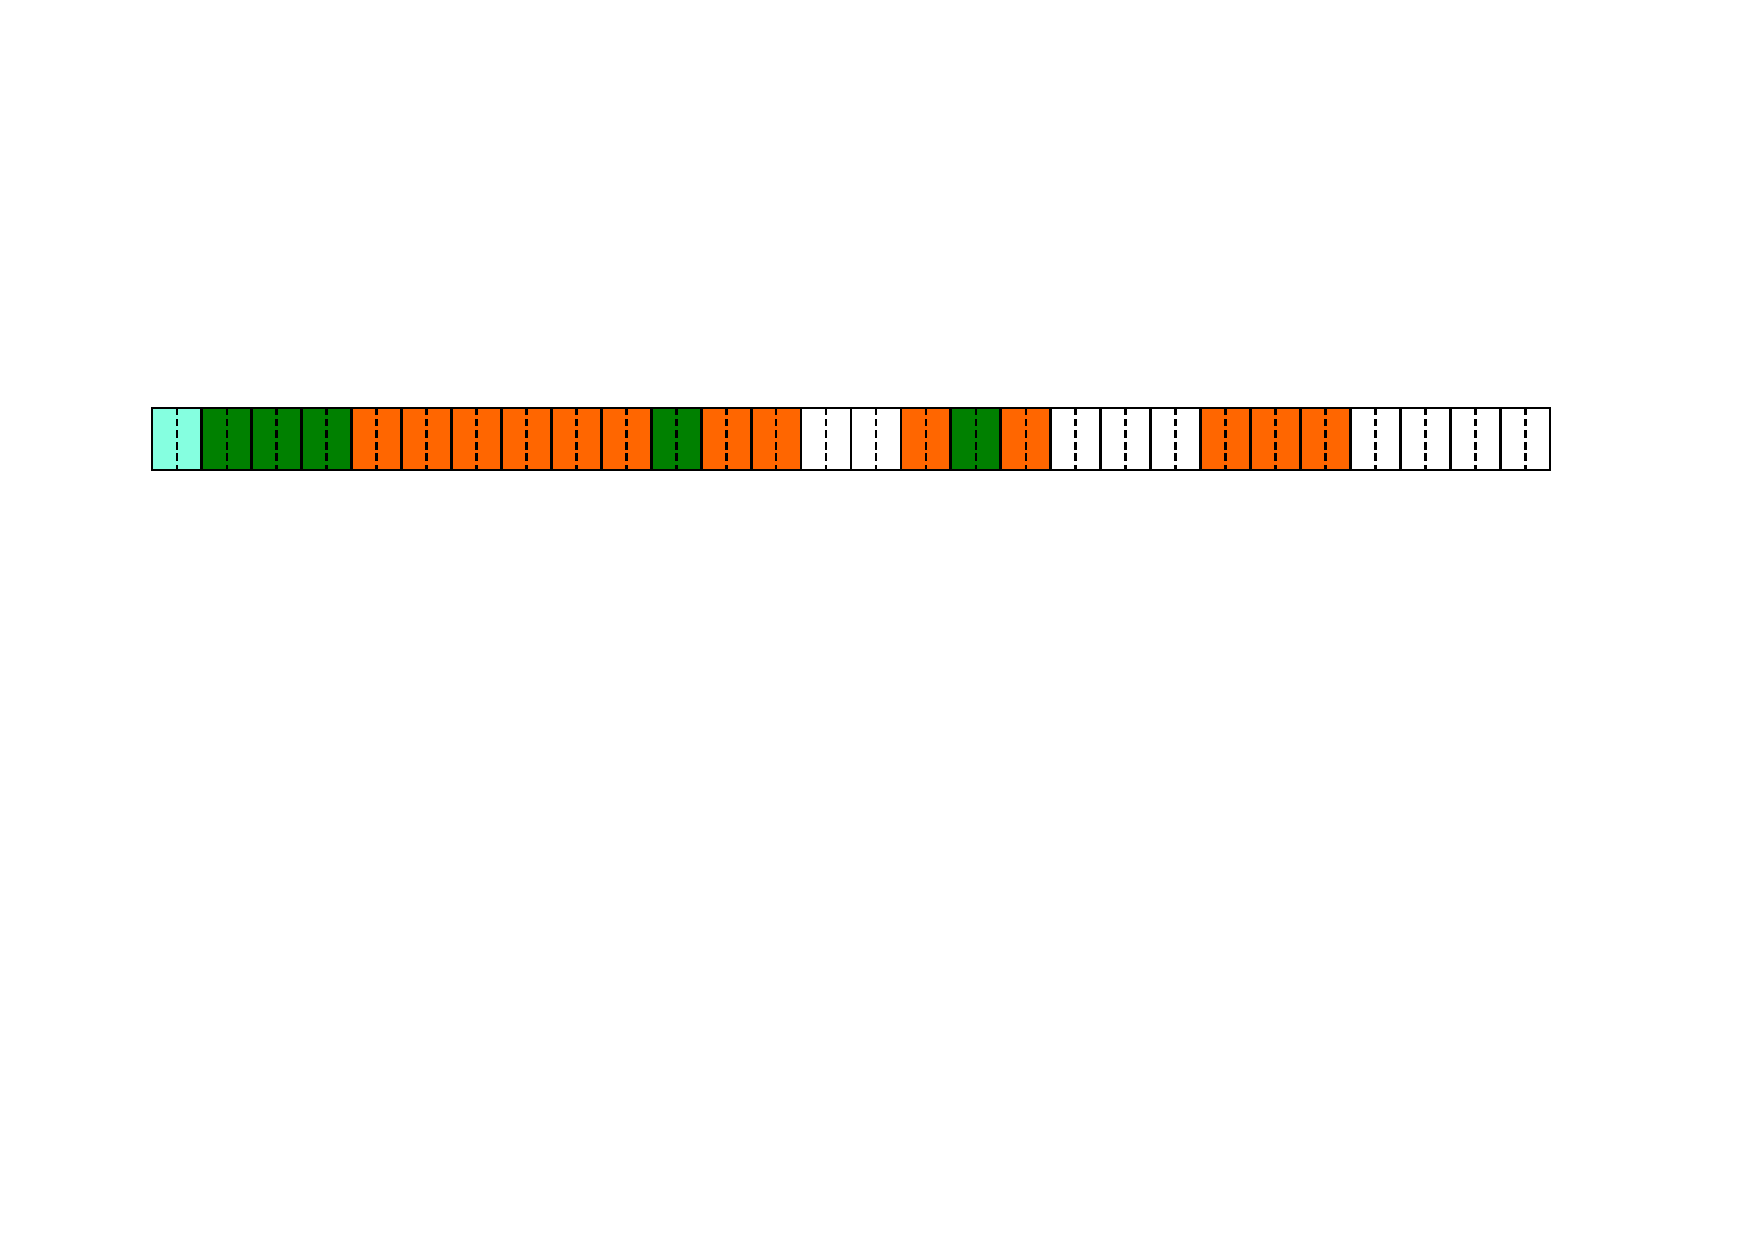
\includegraphics[width=\textwidth]{img/files-1.pdf}
    \caption{A cluster can be seen visually as an array. In this image, for example, we've shown three types of cluster: metadata fixed position (azure), metadata variable position (green), file data (orange), unused space (white).}
\end{figure}

\newpage

\noindent
The following explanation introduces some basic operations on the files to see what happens inside the disks.
\begin{itemize}
    \item \underline{\textbf{Reading}}. To read a file:
    \begin{enumerate}
        \item Access the metadata, variable position (because it contains the folder structure), to locate its block;
        \item Access the blocks to read the contents of the file.
    \end{enumerate}
    \begin{figure}[!htp]
        \centering
        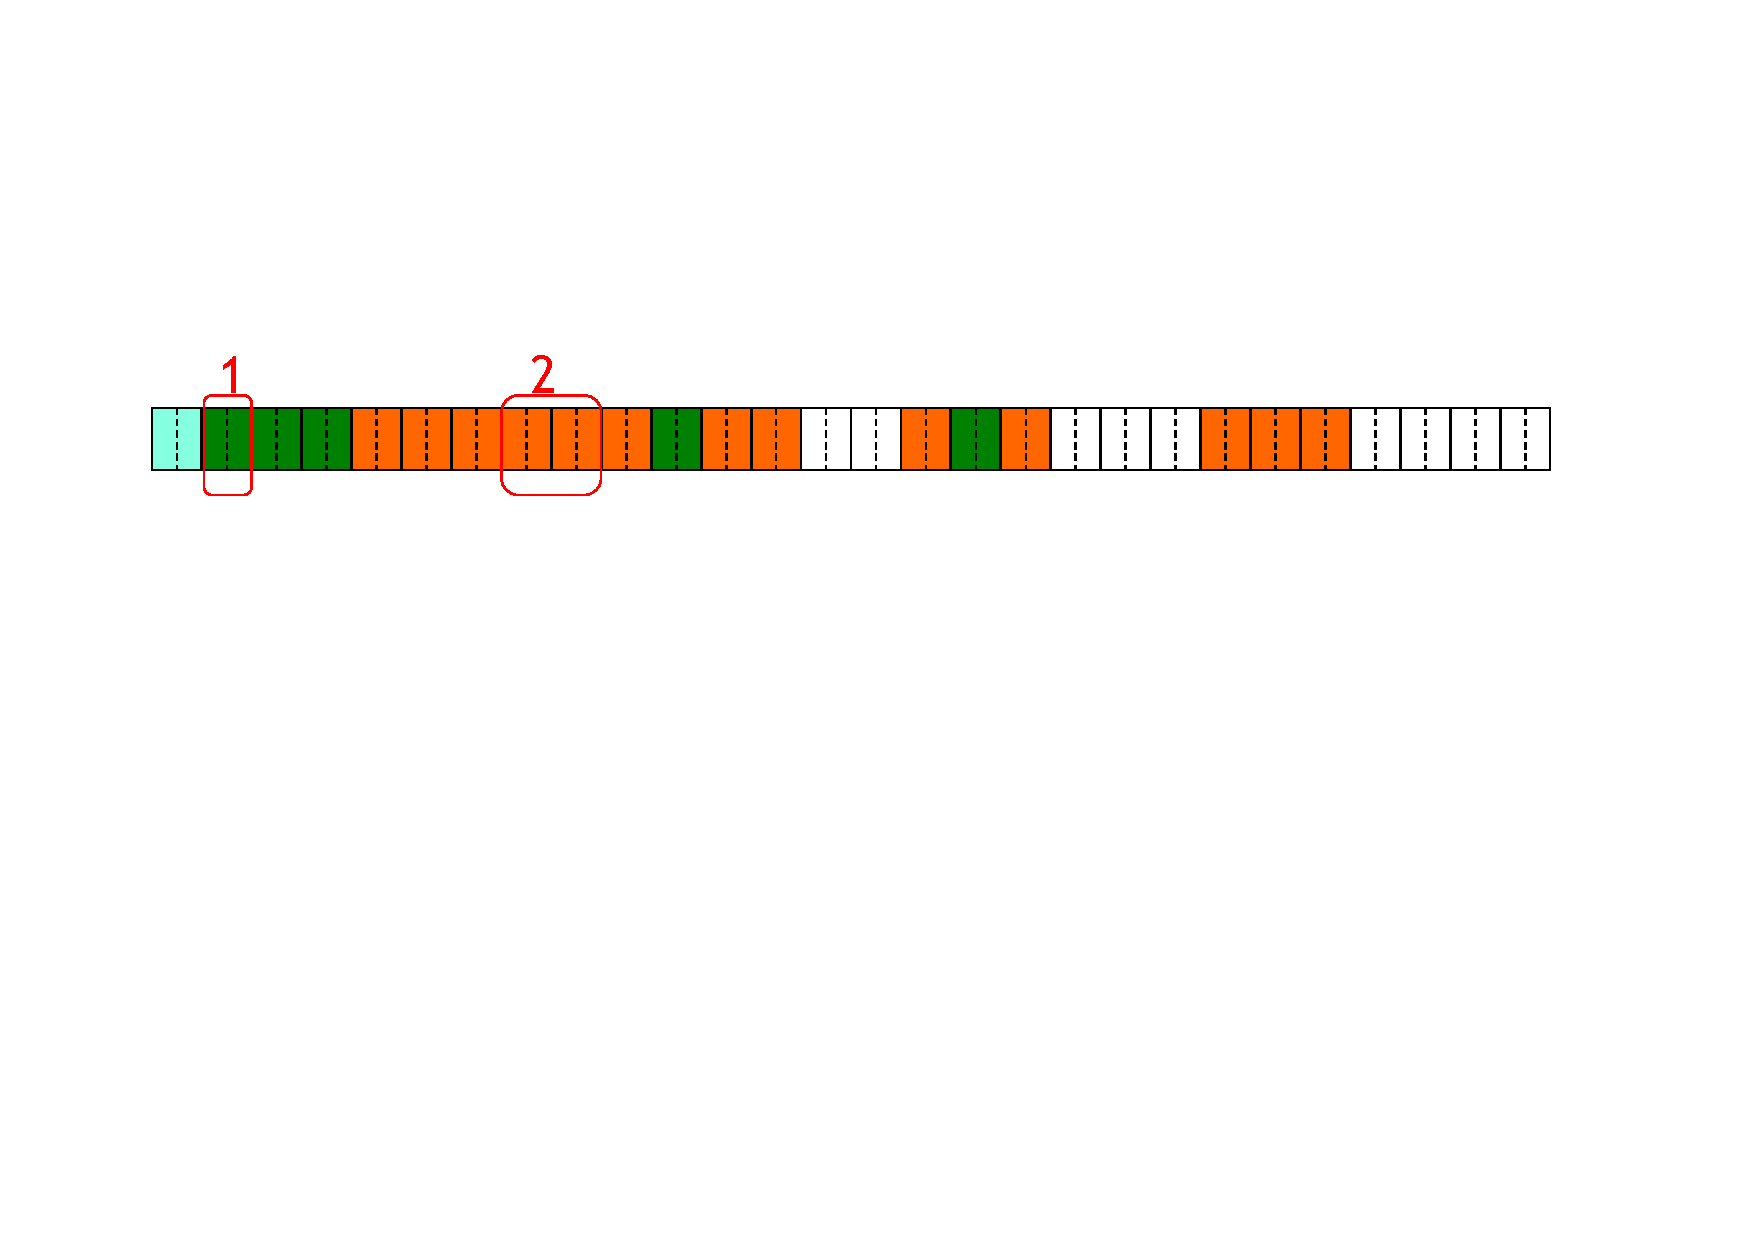
\includegraphics[width=\textwidth]{img/files-2.pdf}
    \end{figure}

    \item \underline{\textbf{Writing}}. To write a file:
    \begin{enumerate}
        \item Access the metadata, variable position (because it contains the folder structure), to find free space.
        \item Write the data in the allocated blocks (cluster type: unused space).        
    \end{enumerate}
    \begin{figure}[!htp]
        \centering
        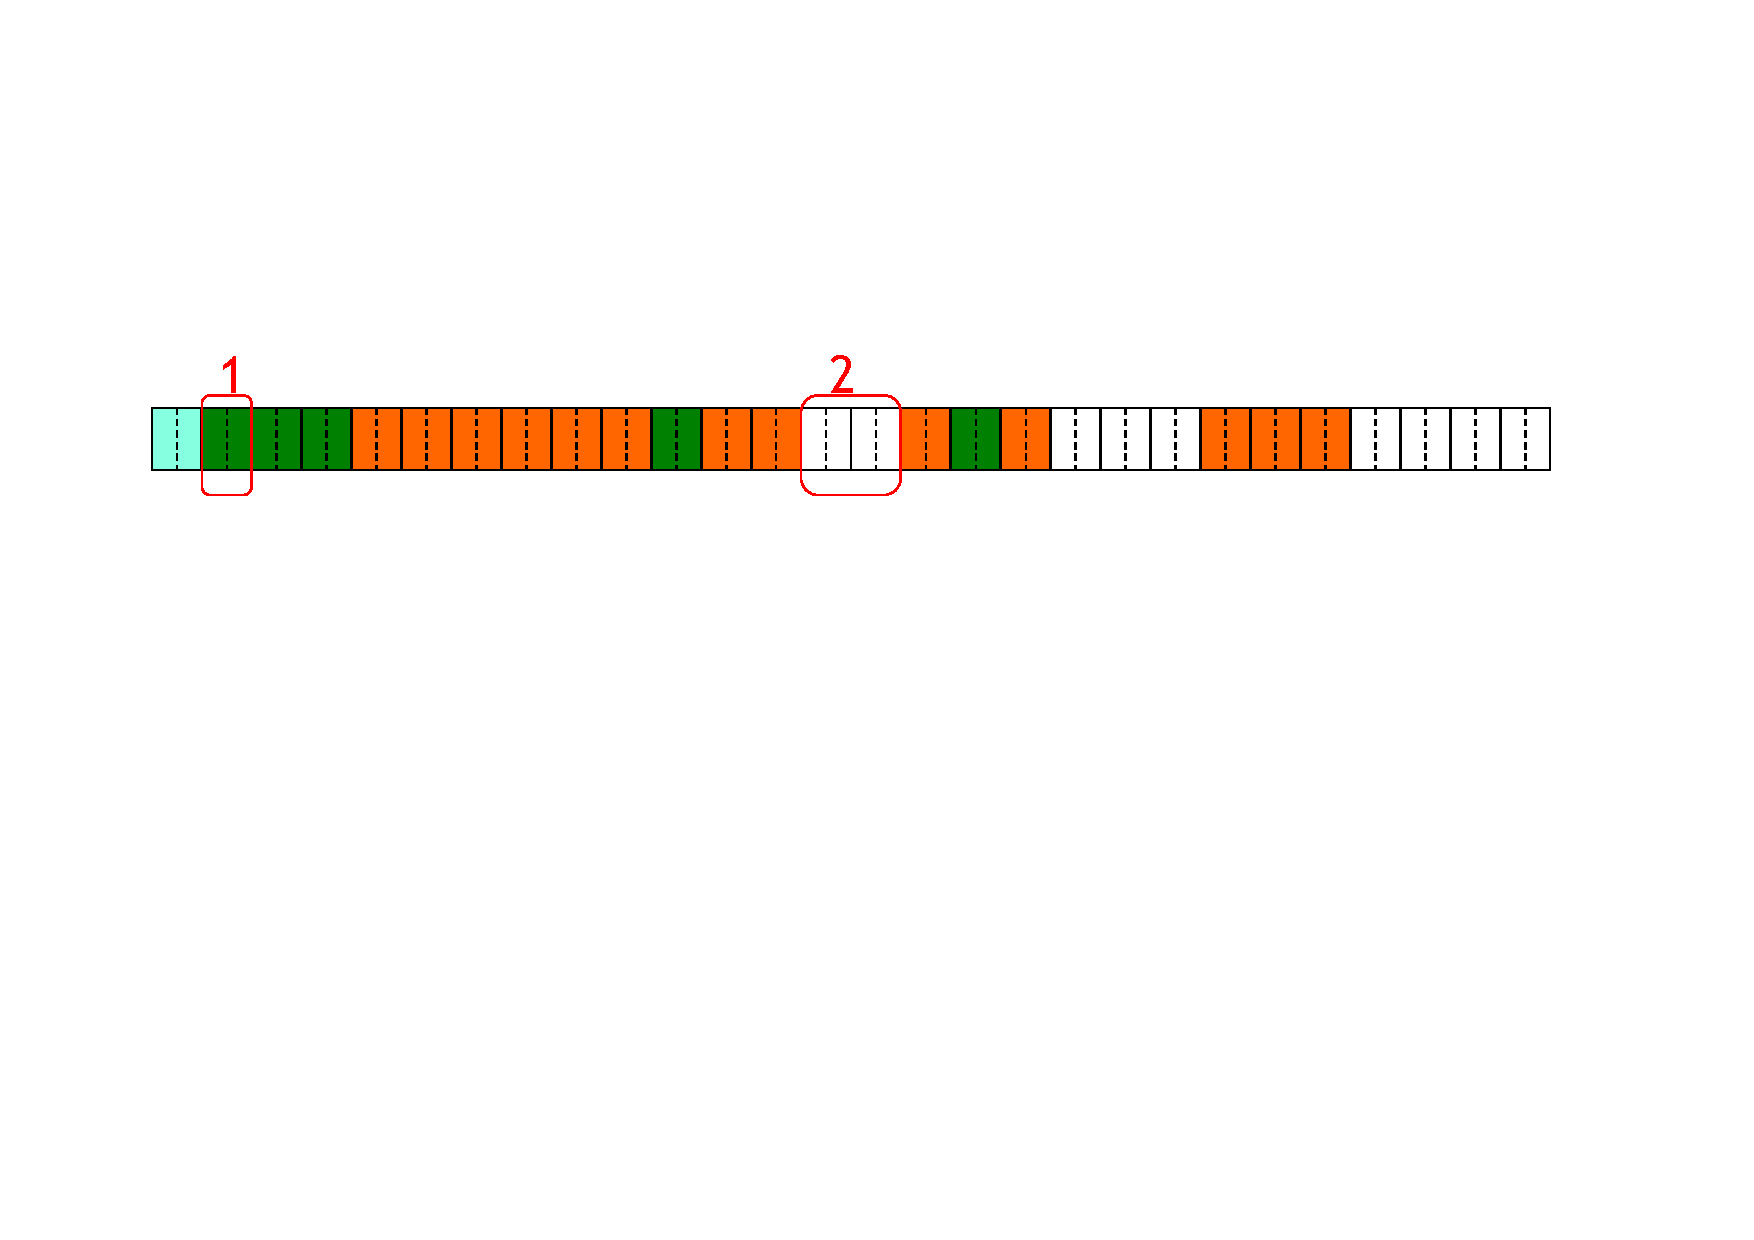
\includegraphics[width=\textwidth]{img/files-3.pdf}
    \end{figure}

    Since the \emph{file system can only access clusters}, the \textbf{actual space taken up by a file on a disk is always a multiple of the cluster size}. Given:
    \begin{itemize}
        \item $s$, the \emph{file size}
        \item $c$, the \emph{cluster size}
    \end{itemize}
    Then the \definition{actual size on the disk $a$} can be calculated as:
    \begin{equation}
        a = \mathrm{ceil}\left(\dfrac{s}{c}\right) \times c
    \end{equation}
    Where $\mathrm{ceil}$ rounds a number \underline{up} to the nearest integer. It's also possible to calculate the \textbf{amount of disk space wasted by organising the file into clusters} (\definition{wasted disk space $w$}):
    \begin{equation}
        w = a - s
    \end{equation}
    A formal way to refer to wasted disk space is \definition{internal fragmentation} of files.
    \newpage
    \begin{examplebox}[: internal fragmentation]
        \begin{itemize}
            \item File size: 27 byte
            \item Cluster size: 8 byte
        \end{itemize}
        The \emph{actual size} on the disk is:
        \begin{equation*}
            a = \mathrm{ceil}\left(\dfrac{27}{8}\right) \cdot 8 = \mathrm{ceil}\left(3.375\right) \cdot 8 = 4 \cdot 8 = 32 \text{ byte}
        \end{equation*}
        And the internal fragmentation $w$ is:
        \begin{equation*}
            w = 32 - 27 = 5 \text{ byte}
        \end{equation*}
    \end{examplebox}

    \item \underline{\textbf{Deleting}}. To delete a file:
    \begin{enumerate}
        \item Just update the metadata, variable position (because it contains the folder structure), to say that the blocks where the file was stored are no longer used by the OS.
    \end{enumerate}
    \textbf{Deleting a file never actually deletes the data on the disk}: if a new file is written to the same clusters, the old data is replaced by the new.
    \begin{figure}[!htp]
        \centering
        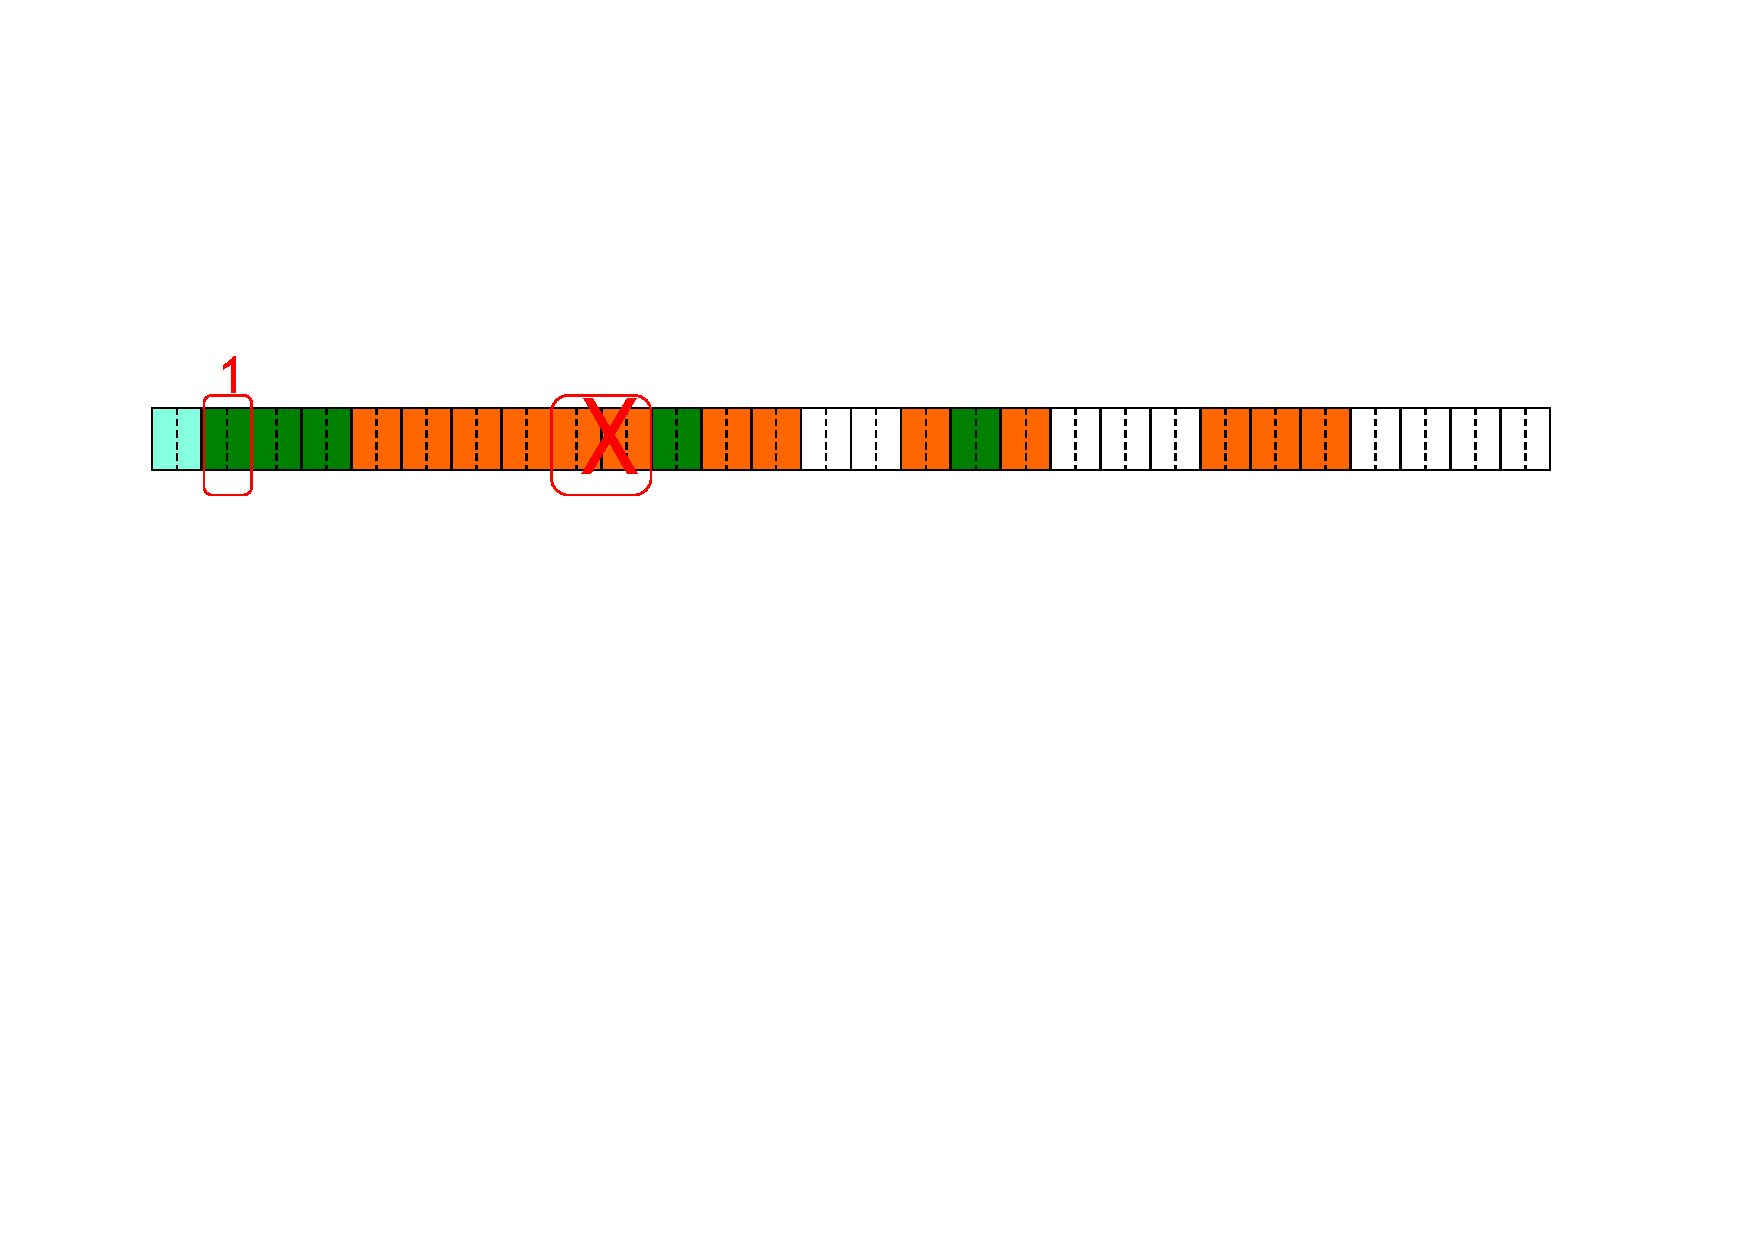
\includegraphics[width=\textwidth]{img/files-4.pdf}
    \end{figure}
    
    \item \underline{\textbf{External fragmentation}}. As the disk's life evolves, there might \textbf{not be enough space to store a file contiguously}.
    
    In this case, the file is split into smaller chunks and inserted into the free clusters spread over the disk.
    
    The effect of \textbf{splitting a file into non-contiguous clusters} is called \definition{external fragmentation}.
    \begin{figure}[!htp]
        \centering
        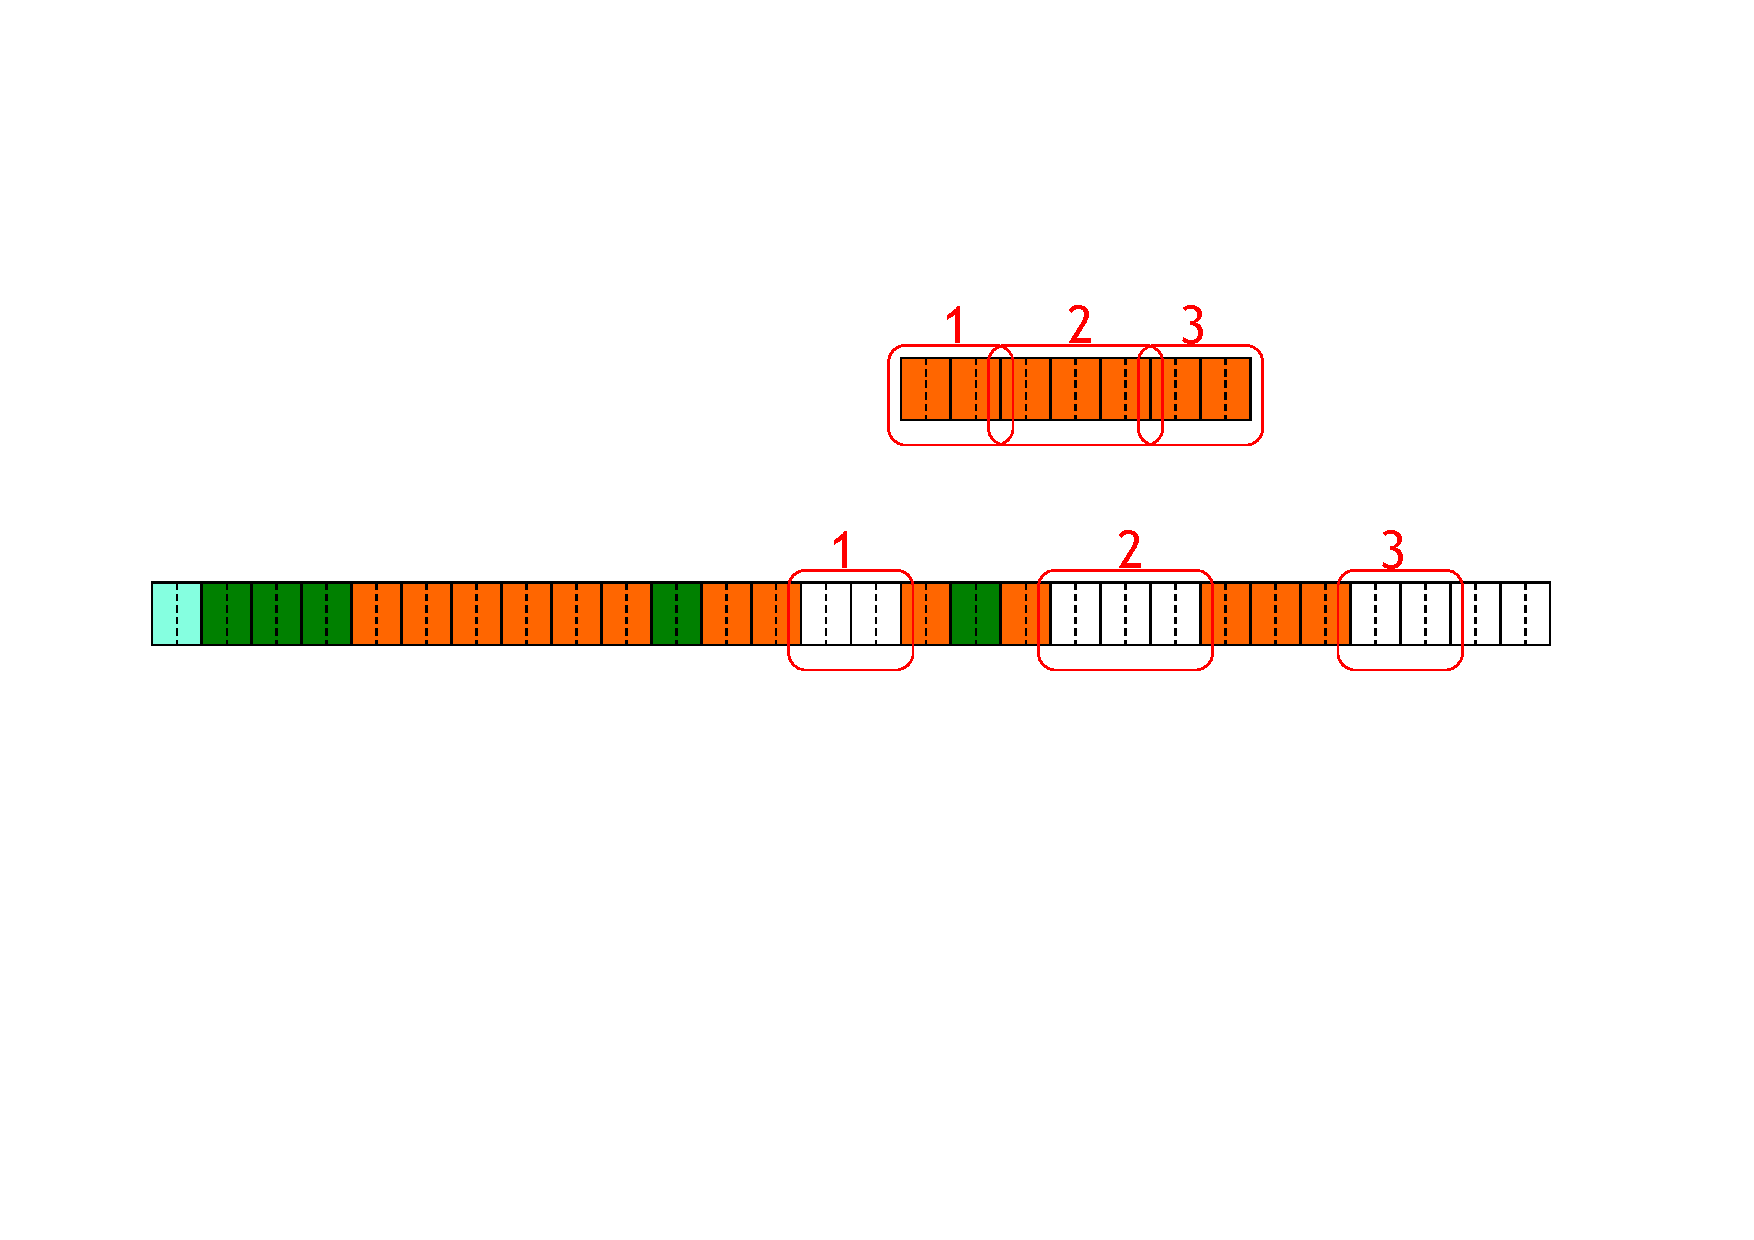
\includegraphics[width=\textwidth]{img/files-5.pdf}
    \end{figure}
\end{itemize}

\newpage

\paragraph{HDD}

A \definition{Hard Disk Drive (HDD)} is a \textbf{data storage device that uses rotating disks (platters) coated with magnetic material}.

\highspace
\textbf{Data is read randomly}, meaning individual data blocks can be stored or retrieved in any order rather than sequentially.

\highspace
An HDD consists of one or more rigid (\emph{hard}) rotating disks (platters) with magnetic heads arranged on a moving actuator arm to read and write data to the surfaces.

\begin{figure}[!htp]
    \centering
    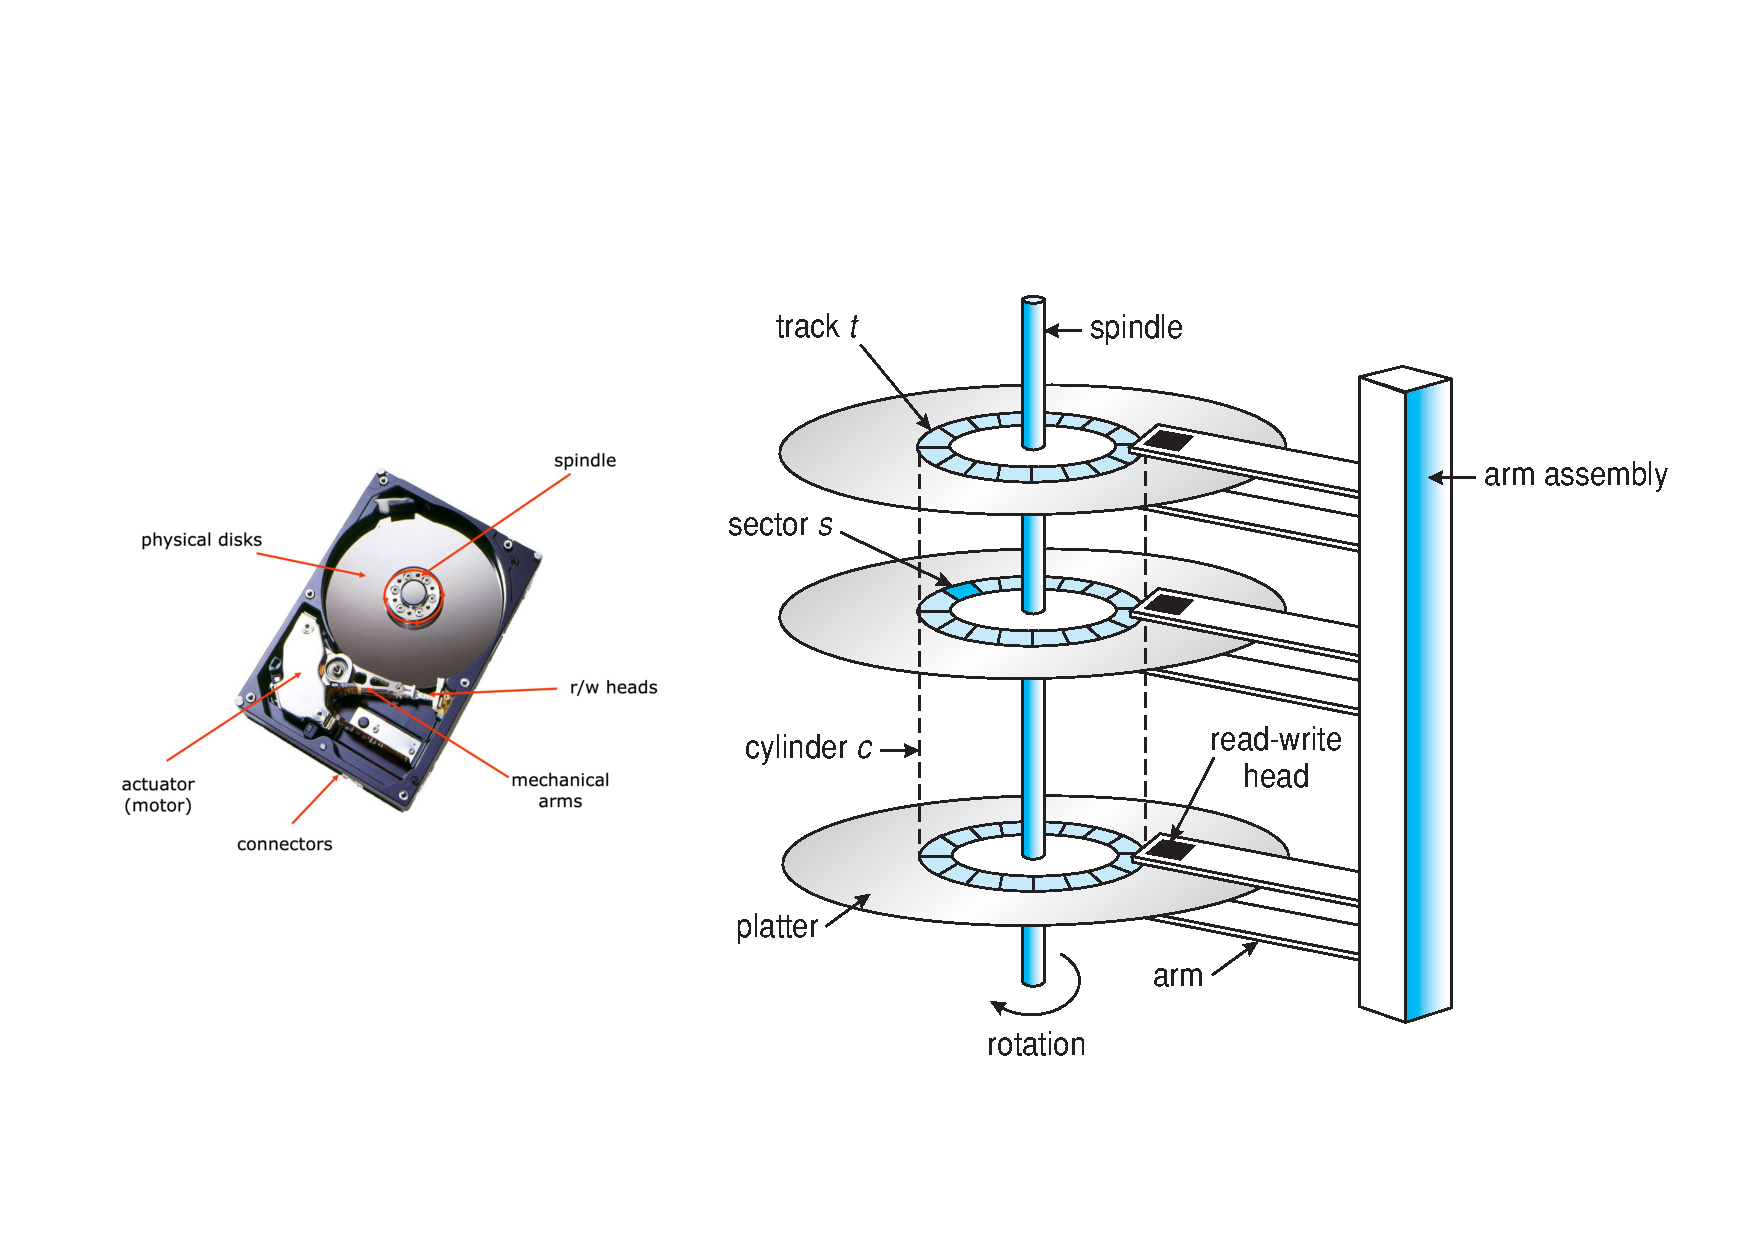
\includegraphics[width=\textwidth]{img/files-6.pdf}
    \caption{Hard Drive Disk anatomy.}
\end{figure}

\noindent
Externally, hard drives expose a large number of \textbf{sectors} (blocks):
\begin{itemize}
    \item Typically, 512 or 4096 bytes.
    \item Individual \textbf{sector writes} are \textbf{atomic}.
    \item Multiple sectors write it may be interrupted (\definition{torn write}\footnote{Torn writes happen when only part of a multi-sector update is written successfully to disk.}).
\end{itemize}
The geometry of the drive:
\begin{itemize}
    \item The sectors are arranged into \textbf{tracks}.
    \item A \textbf{cylinder} is a particular track on multiple platters.
    \item Tracks are arranged in concentric circles on \textbf{platters}.
    \item A disk may have multiple double-sided platters.
\end{itemize}
The \textbf{driver motor spins the platters at a constant rate}, measured in \definition{Revolutions Per Minute (RPM)}.

\newpage

\begin{figure}[!htp]
    \centering
    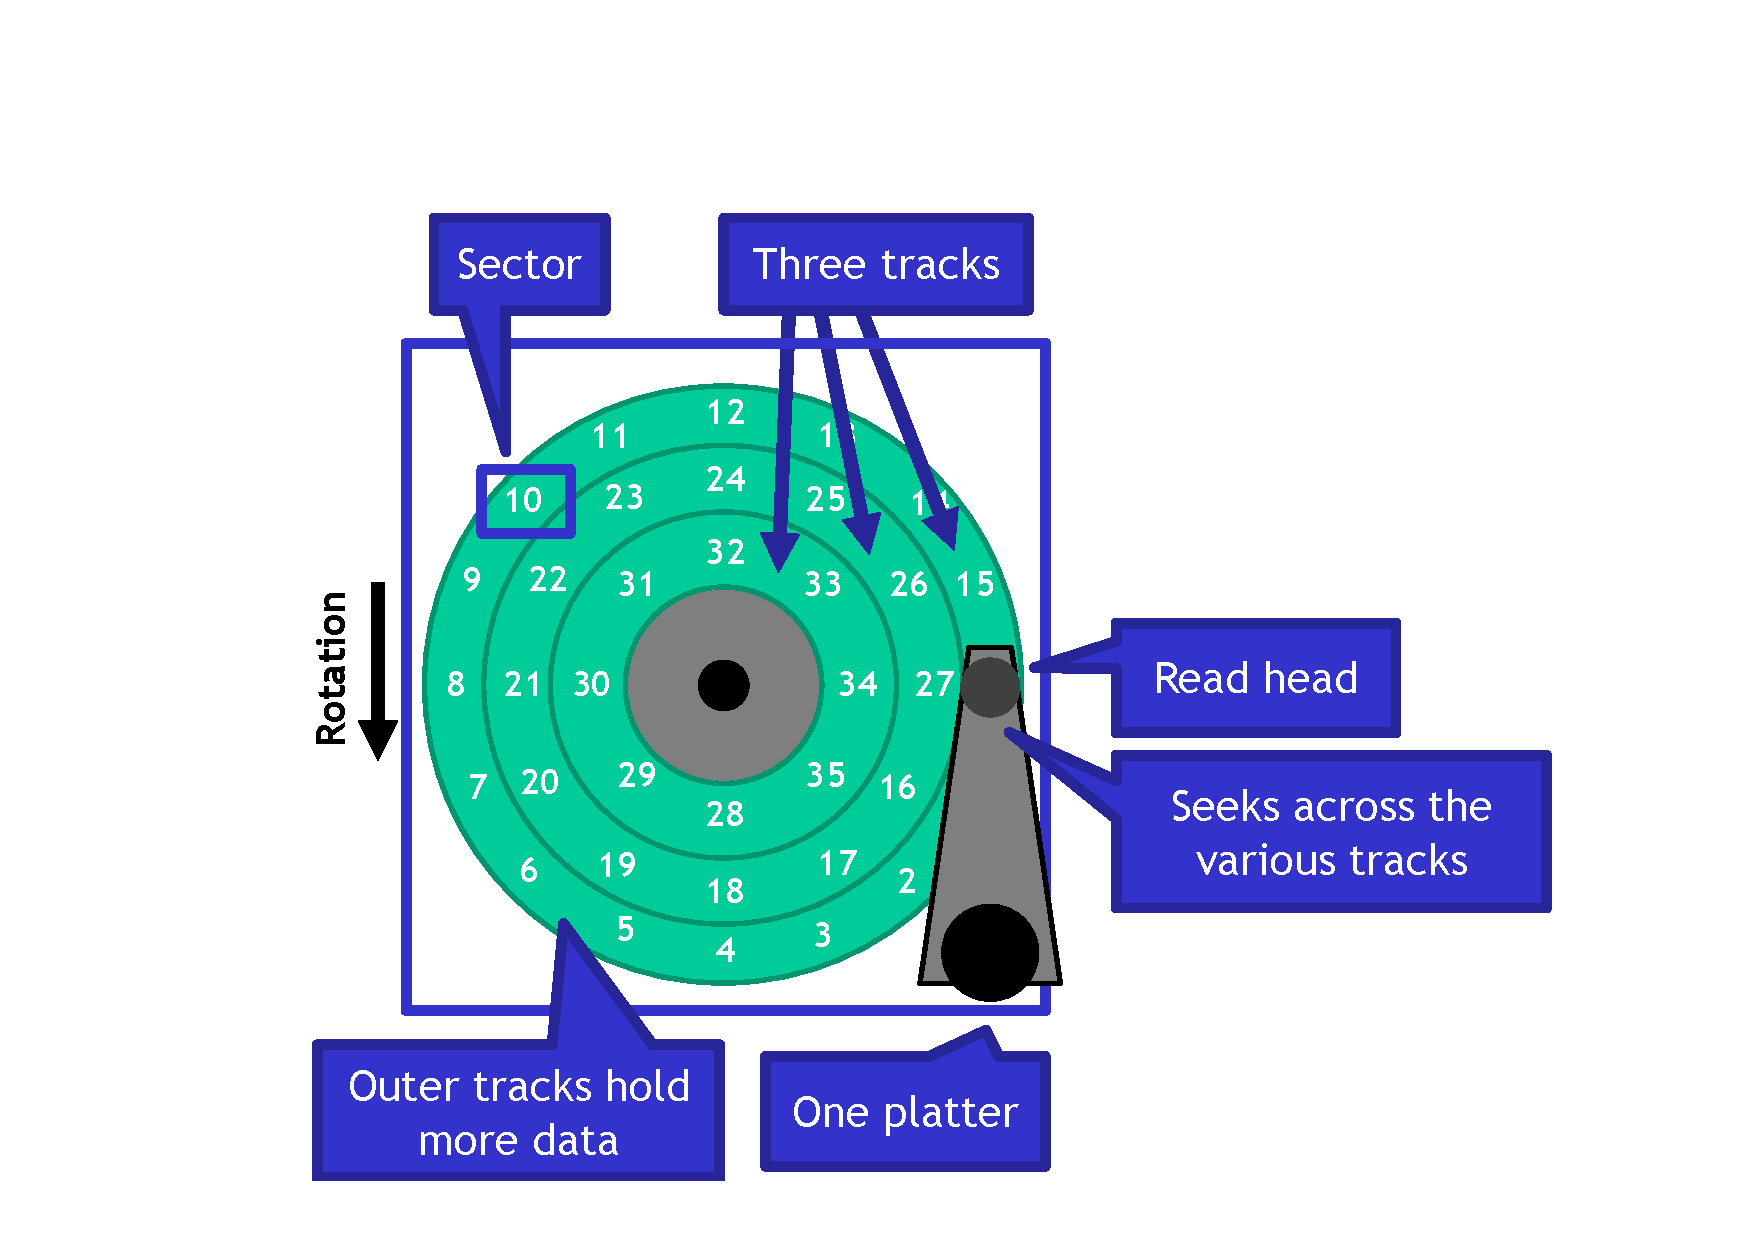
\includegraphics[width=.8\textwidth]{img/files-7.pdf}
    \caption{Example of HDD geometry.}
\end{figure}

Given the architecture of the HDD, there are \textbf{four types of delay}:
\begin{itemize}\label{four types of hdd delay}
    \item \definition{Rotational Delay} is the \textbf{time to rotate the desired sector to the read head}, and it's related to RPM.
    \item \definition{Seek Delay} is the \textbf{time to move the read head to a different track}.
    \item \definition{Transfer time} is the \textbf{time to read or write bytes}.
    \item \definition{Controller Overhead} is the \textbf{overhead for the request management}.
\end{itemize}

\newpage

\paragraph{SSD}

\paragraph{RAID}

\subsubsection{Networking (architecture and technology)}\label{subsubsection: Networking (architecture and technology)}


    %%%%%%%%%%%%%%%%%%%%%%%%%%%%
    % Software Infrastructures %
    %%%%%%%%%%%%%%%%%%%%%%%%%%%%
    \section{Software Infrastructure}

\subsection{Virtualization}

\subsubsection{What is a Virtual Machine?}

A \definition{Virtual Machine (VM)} is a \textbf{logical abstraction} able to \textbf{provide a virtualized execution environment}. More specifically, a VM:
\begin{itemize}
    \item Provides identical software behavior
    \item Consists in a combination of physical machine and virtualizing software
    \item May appear as different resources than physical machine
    \item May result in different level of performances
\end{itemize}
Exists two type of Virtual Machine: Process VM (page \pageref{Process VM}) and System VM (page \pageref{System VM}).

\highspace
\begin{flushleft}
    \textcolor{Green3}{\faIcon{question-circle} \textbf{What's the difference between a physical machine and a virtual machine?}}
\end{flushleft}
First of all, the \textbf{physical machine} is the computer that can \textbf{\emph{host}} $n$ \textbf{virtual machines}. 

\highspace
Furthermore, every VM is based on hypervisor software (also known as a virtual machine manager or monitor VMM, page \pageref{subsubsection: Virtual Machine Managers (VMM)}). The hypervisor runs as an application on the host operating system (hosted hypervisor) or rests directly on the hardware of the physical machine (bare-metal hypervisor) and manages the hardware resources provided by the host system. The \textbf{hypervisor software creates an abstraction layer between physical hardware and virtual machines}. \textbf{Each VM runs isolated from the host system and other guest systems on its own virtual environment}. This is referred to as encapsulation. 

\highspace
Processes within a virtual machine do not affect the host or other VMs on the same hardware.

\highspace
So, to sum up:
\begin{enumerate}
    \item \textbf{Physical machines} are the computers that can \textbf{\emph{host}} $n$ \textbf{virtual machines}.
    
    \item Each \textbf{physical machine has a hypervisor (VMM)} already enabled or asleep on the hardware. \textbf{It manages the resources made available by the physical machine}.
    
    \item Each \textbf{virtual machine has its own virtual environment}, so they are \textbf{encapsulated}, \textbf{isolated environments.} 
    
    Obviously, the statement is not true if there is a \dquotes{\emph{virtual machine escape attack}}, but we don't count those extreme cases.\cite{wu2017access}
\end{enumerate}

\newpage

\begin{figure}[!htp]
    \centering
    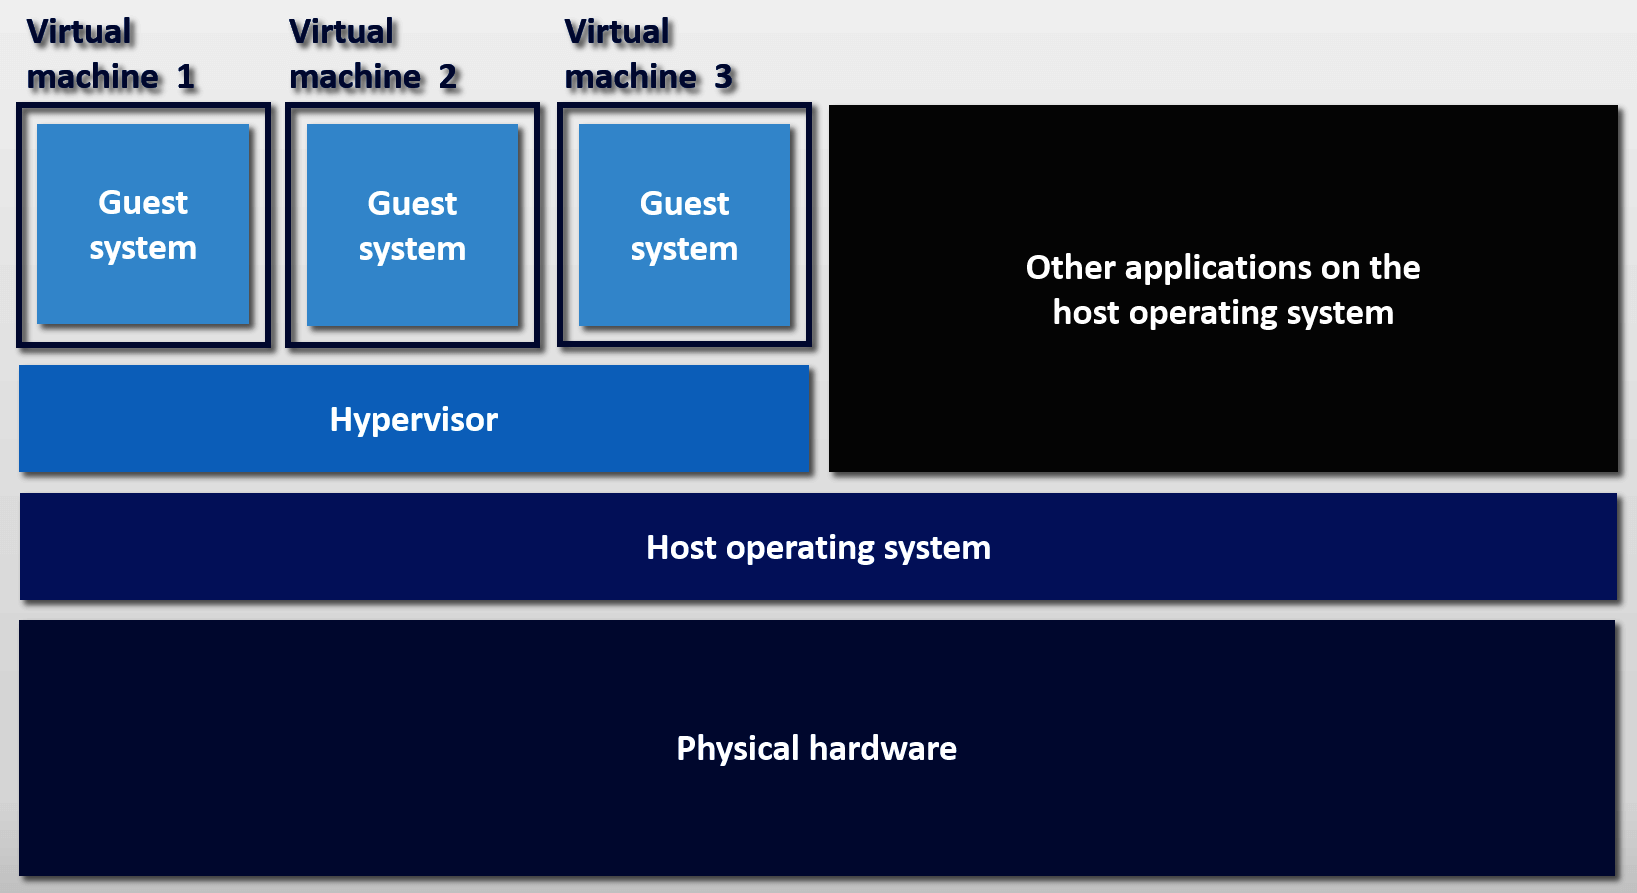
\includegraphics[width=\textwidth]{img/vm-1.png}
    \caption{Operating system view if there are VMs in the physical machine (source: \href{https://www.ionos.co.uk/digitalguide/server/know-how/virtual-machines/}{ionos}).}
\end{figure}

\noindent
A little terminology about \emph{host} and \emph{guest}:
\begin{itemize}
    \item \textbf{\underline{Host}}: the underlying platform supporting the environment/system.
    \item \textbf{\underline{Guest}}: the software that runs in the Virtual Machine environment as the guest.
\end{itemize}

\newpage

\paragraph{Process VM}\label{Process VM}

A \definition{Process Virtual Machine}, sometimes called an application virtual machine, or Managed Runtime Environment (MRE), \textbf{runs as a normal application inside a host OS and supports a single process}. 

\highspace
The \textbf{Virtual Machine is created when that process begins and destroyed when it ends}. A good example is the Java Virtual Machine JVM (see more \href{https://en.wikipedia.org/wiki/Java_virtual_machine}{here}).

\highspace
The purpose of a process VM is to execute a computer program in a platform-independent environment, meaning it can run on a variety of hardware or software.

\highspace
The virtualizing software:
\begin{itemize}
    \item is placed at the ABI\footnote{An \definition{Application Binary Interface (ABI)} corresponds to \dquotes{\emph{Operating system machine level}}.}, on top of the OS/hardware combination.
    \item emulates both user-level instructions and operating system calls.
    \item is usually called Runtime Software.
\end{itemize}

\begin{figure}[!htp]
    \centering
    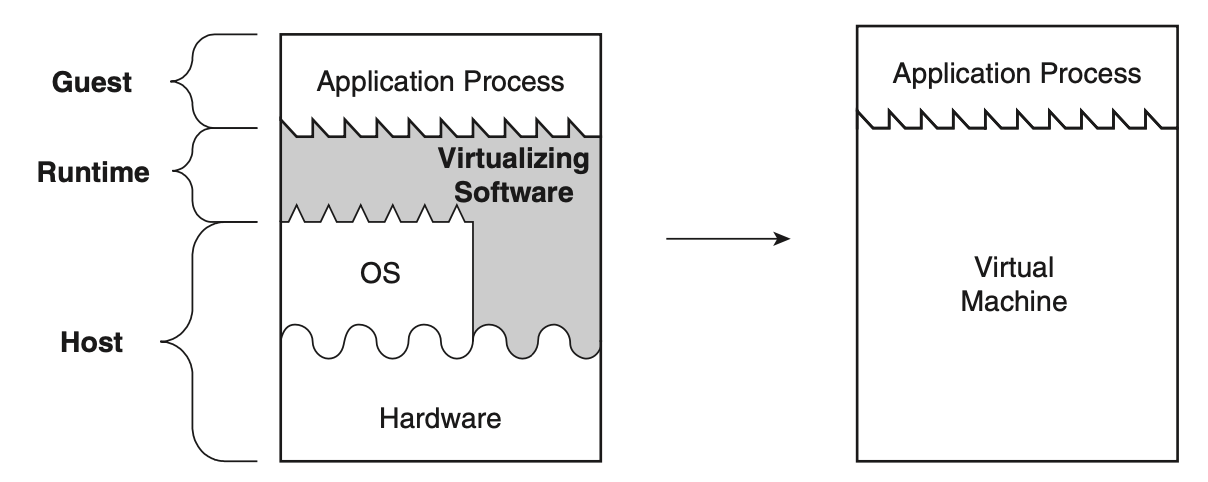
\includegraphics[width=.9\textwidth]{img/vm-2.png}
    \caption{Process VM.}
\end{figure}

\newpage

\paragraph{System VM}\label{System VM}

\definition{System Virtual Machine}s are substitutes for real machines and \textbf{provide all the functionalities of an actual operating system}. It provides operating system running in it access to underlying hardware resources (networking, I/O, GUI).

\highspace
With a system VM, the hypervisor will access the underlying machine's resources, giving the user the same capabilities the host device offers.

\highspace
The \textbf{virtualization software is called \definition{Virtual Machine Monitor (VMM)}}.

\begin{figure}[!htp]
    \centering
    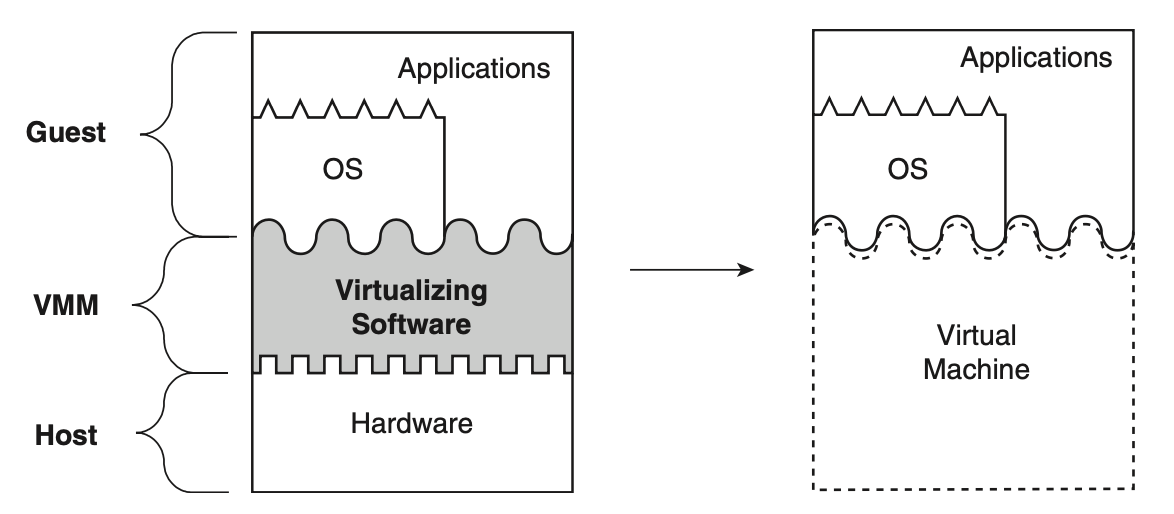
\includegraphics[width=.9\textwidth]{img/vm-3.png}
    \caption{System VM.}
\end{figure}

\newpage

\subsubsection{Virtualization Implementation}

\subsubsection{Virtual Machine Managers (VMM)}\label{subsubsection: Virtual Machine Managers (VMM)}

\paragraph{Paravirtualization}

\paragraph{Full virtualization}

\paragraph{Containers}

    \subsection{Computing Architectures}

    %%%%%%%%%%%
    % Methods %
    %%%%%%%%%%%
    \section{Methods}

\subsection{Reliability and availability of datacenters}

\subsubsection{Introduction}\label{subsubsection: introduction - dependability}

\definition{Dependability} \textbf{measures how much we trust a system}. More technically, it is the \textbf{ability of a system to perform its functionality while exposing}:
\begin{itemize}
    \item \textbf{Reliability}. Continuity of correct service.
    \item \textbf{Availability}. Readiness for correct service.
    \item \textbf{Maintainability}. Ability for easy maintenance.
    \item \textbf{Safety}. Absence of catastrophic consequences.
    \item \textbf{Security}. Confidentiality and integrity of data.
\end{itemize}

\highspace
\begin{flushleft}
    \textcolor{Green3}{\faIcon{question-circle} \textbf{Ok, but why should we be interested in dependability?}}
\end{flushleft}
During the implementation of a product, there is much effort to make sure that the implementation:
\begin{itemize}
    \item matches specifications,
    \item fulfils requirements,
    \item meets constraints,
    \item optimizes selected parameters (such as performance, energy, etc.).
\end{itemize}
Nevertheless, even if all the above aspects are satisfied, the systems fail because something broke! The causes can be multiple: defects, process variation, degraded transistors, radiation, noise, design errors, software bugs, OS bugs, malicious attacks, and human errors.

\highspace
Then, \textbf{dependability is essential} to check how much we can trust a system despite the effects of failure. If we are not convinced, consider that \textbf{a failure may have high costs if it impacts economic losses or physical damage}. Not only that, a single system failure may affect a large number of people and may cause information loss with a high consequent recovery cost. For the previous reasons, the systems that are not dependable are likely \emph{not to be used or adopted}.

\highspace
\begin{flushleft}
    \textcolor{Green3}{\faIcon{question-circle} \textbf{It seems very important, so when should we think about dependability?}}
\end{flushleft}
Consistently, both at \emph{design-time} to:
\begin{itemize}
    \item Analyze the system under design;
    \item Measure dependability properties;
    \item Modify the design if required;
\end{itemize}
And \emph{runtime} to:
\begin{itemize}
    \item Detect malfunctions;
    \item Understand causes;
    \item React.
\end{itemize}
Furthermore, the failures in development should be avoided, and the design should take failures into account and guarantee that control and safety are achieved when failures occur. The effects of such failures should be predictable and deterministic, not catastrophic!

\highspace
\begin{flushleft}
    \textcolor{Green3}{\faIcon{question-circle} \textbf{Always think about dependability, but where should it be applied?}}
\end{flushleft}
In the past, dependability was relevant only for \emph{safety-critical} and \emph{mission-critical} application environments: space, nuclear, and avionics. Note that:
\begin{itemize}
    \item \definition{Mission-critical systems} are architectures where a \textbf{failure} during operation \textbf{can have severe or irreversible effects on the mission the system is carrying out} (for example, satellites, surveillance drones, unmanned vehicles, etc.).
    
    \item \definition{Safety-critical systems} are architectures where a \textbf{failure} during operation can \textbf{directly threaten human life} (for example, aircraft control systems, medical instrumentation, railway signaling, nuclear reactor control systems).
\end{itemize}
However, in the computing infrastructures, the \textbf{downtime is the enemy of every data center}! So it is important to consider the dependability in each scenario in order to guarantee that everything works properly.

\highspace
\begin{flushleft}
    \textcolor{Green3}{\faIcon{question-circle} \textbf{Finally, how to provide dependability?}}
\end{flushleft}
It depends on the paradigm adopted:
\begin{itemize}
    \item The \definition{Avoidance} paradigm is a \textbf{conservative design}; it implements a design validation, has some detailed hardware and software tests, and is an error avoidance-driven approach.

    \item The \definition{Tolerance} paradigm is an \textbf{error detection during system operation}; it implements online monitoring; if there is an error, it gives diagnostic solutions and has a self-recovery and self-repair.
\end{itemize}
To apply these paradigms, it is necessary to work at the:
\begin{itemize}
    \item \textbf{Technological level} to design and manufacture by employing reliable/robust components.

    \item \textbf{Architectural level} to integrate standard components using solutions that allow to manage the occurrence of failures.

    \item \textbf{Software/Application level} to develop solutions in the algorithms or in the operating systems that mask and recover from the occurrence of failures. This guarantees high dependability, high cost, and reduced performance.
\end{itemize}
Finally, all of these solutions have a common \textbf{cost and reduced performance}.

\newpage

\subsubsection{Reliability and Availability}

Dependability contains the properties of reliability and availability (see page \pageref{subsubsection: introduction - dependability}).

\highspace
\begin{definitionbox}[: Reliability]\index{Reliability}
    The \textbf{ability} of a system or component \textbf{to perform its required functions under stated conditions for a specified period of time}.
\end{definitionbox}

\highspace
We can also calculate the \textbf{probability} that the \textbf{system will operate correctly} in a specified operating environment \underline{until} time $t$:
\begin{equation}\label{eq: reliability probability}
    R\left(t\right) = P\left(\text{not failed during } \left[0,t\right]\right)
\end{equation}
(assuming it was operating at time $t=0$). Note that the time $t$ is essential because it is often \textbf{used to characterize systems in which even small periods of incorrect behaviour are unacceptable} (e.g. impossibility to repair). For example, if a system needs to work for slots of ten hours at a time, then ten hours is the reliability target.

\highspace
As a consequence, the \definition{unreliability $Q\left(t\right)$} can be calculated as follows:
\begin{equation}
    Q\left(t\right) = 1 - R\left(t\right)
\end{equation}
The reliability probability is a \textbf{non-increasing function} ranging from $1$ to $0$ over $\left.\left[0, +\infty\right.\right)$.
\begin{equation}
    \begin{array}{rcl}
        R\left(0\right) &=& 1 \\ [.5em]
        \lim\limits_{t \rightarrow +\infty} R\left(t\right) &=& 0 \\ [.5em]
        f\left(x\right) &=& -\dfrac{\mathrm{d}R\left(t\right)}{\mathrm{d}t}
    \end{array}
\end{equation}
We can observe that the probability of the reliability at the time zero is equal to one because we assume it was operating at time zero. Furthermore, the reliability probability function goes to zero when the time goes to infinity.

\highspace
\begin{definitionbox}[: Availability]\index{Availability}
    The degree to which a system or component is \textbf{operational and accessible when required for use}. It can be calculated as follows:
    \begin{equation}
        \text{Availability } = \dfrac{\text{Uptime}}{\left(\text{Uptime } + \text{ Downtime}\right)}
    \end{equation}
\end{definitionbox}

\highspace
The \textbf{main difference} between reliability and availability is that \textbf{reliability does not break down}, and \textbf{availability works when needed}, even if it breaks down.

\highspace
Finally, we calculate the \textbf{probability that the system will be operational at time} $t$ as follows:
\begin{equation}
    A\left(t\right) = P\left(\text{not failed at time } t\right)
\end{equation}
It is ready for service and admits the possibility of brief outages. Finally, of course, the \definition{unavailability} is:
\begin{equation}
    \text{unavailability } = 1-A\left(t\right)
\end{equation}

\highspace
\begin{flushleft}
    \textcolor{Green3}{\faIcon{question-circle} \textbf{What is the relationship between reliability and availability?}}
\end{flushleft}
The \textbf{relationship with the reliability} is that:
\begin{itemize}
    \item When the \textbf{system is not repairable}, the availability and reliability are the same:
    \begin{equation}
        A\left(t\right) = R\left(t\right)
    \end{equation}

    \item In general, the \textbf{reparable systems} have
    \begin{equation}
        A\left(t\right) \ge R\left(t\right)
    \end{equation}
\end{itemize}
However, the relationship is more robust because if a \textbf{system is unavailable}, \textbf{it does not deliver the specified system services}. However, it is possible to have \textbf{systems with low reliability that must be available}. Then, the system failures can be repaired quickly and do not damage data, so the low reliability may not be a problem. The opposite is generally more complex.

\newpage

\begin{flushleft}
    \textcolor{Red2}{\faIcon{chart-bar} \textbf{Metrics}}
\end{flushleft}
Some metrics exist for reliability and availability.
\begin{itemize}
    \item The \definition{Mean Time To Failure (MTTF)} is the mean time before any failure will occur. Moreover, it is calculated as the \textbf{integral of the reliability probability} (eq. \ref{eq: reliability probability}, page \pageref{eq: reliability probability}):
    \begin{equation}
        \texttt{MTTF} = \displaystyle\int_{0}^{\infty} R\left(t\right) \:\mathrm{d}t
    \end{equation}
    
    \item The \definition{Mean Time Between Failures (MTBF)} is the \textbf{mean time between two failures}. It is the relationship between the total operating time and the number of failures.
    \begin{equation}
        \texttt{MTBF} = \dfrac{\text{total operating time}}{\text{number of failures}}
    \end{equation}
    %\newpage
    \begin{figure}[!htp]
        \centering
        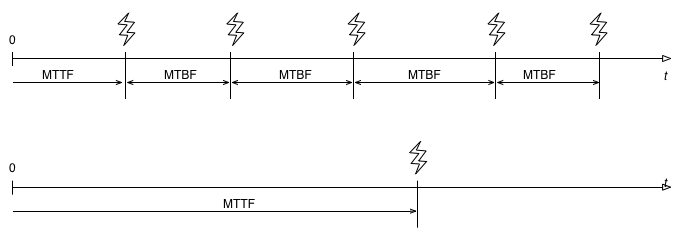
\includegraphics[width=\textwidth]{img/reliability-and-availability-1.png}
    \end{figure}
    
    \item The \definition{Failures In Time (FIT)} is \textbf{another way of reporting \texttt{MTBF}}. It is the number of \textbf{expected failures per one billion hours} ($10^9$) of operation for a device. Then, the \texttt{MTBF} in hours is:
    \begin{equation}
        \texttt{MTBF} = \dfrac{10^{9}}{\texttt{FIT}}
    \end{equation}
    
    \item The \definition{Failure Rate $\lambda$} is the relationship between the number of failures and the total operating time:
    \begin{equation}
        \text{Failure Rate }\lambda = \dfrac{\text{number of failures}}{\text{total operating time}}
    \end{equation}
    If we observe closely, it equals $MTBF^{-1}$, then:
    \begin{equation}
        \texttt{MTBF} = \dfrac{1}{\lambda}
    \end{equation}
\end{itemize}

\newpage

\begin{flushleft}
    \textcolor{Green3}{\faIcon{question-circle} \textbf{How to compute reliability? The Empirical Evaluation}}
\end{flushleft}
In general, Empirical Evaluation is an evaluation method in which results are derived from observation or experiment rather than theory.

\highspace
Regarding reliability, let us consider:
\begin{itemize}
    \item $n_{0}$ independent and statistically identical elements deployed at time $t = 0$ in identical conditions $n\left(0\right) = n_{0}$;

    \item At time $t$, the $n\left(t\right)$ elements do not fail.

    \item Furthermore, $t_1$, $t_2$, $\dots$, $t_{n_{0}}$ are the times of failure of the $n_0$ elements. Note that the times to failure are independent occurrences of the random quantity $T$.
\end{itemize}

\begin{figure}[!htp]
    \centering
    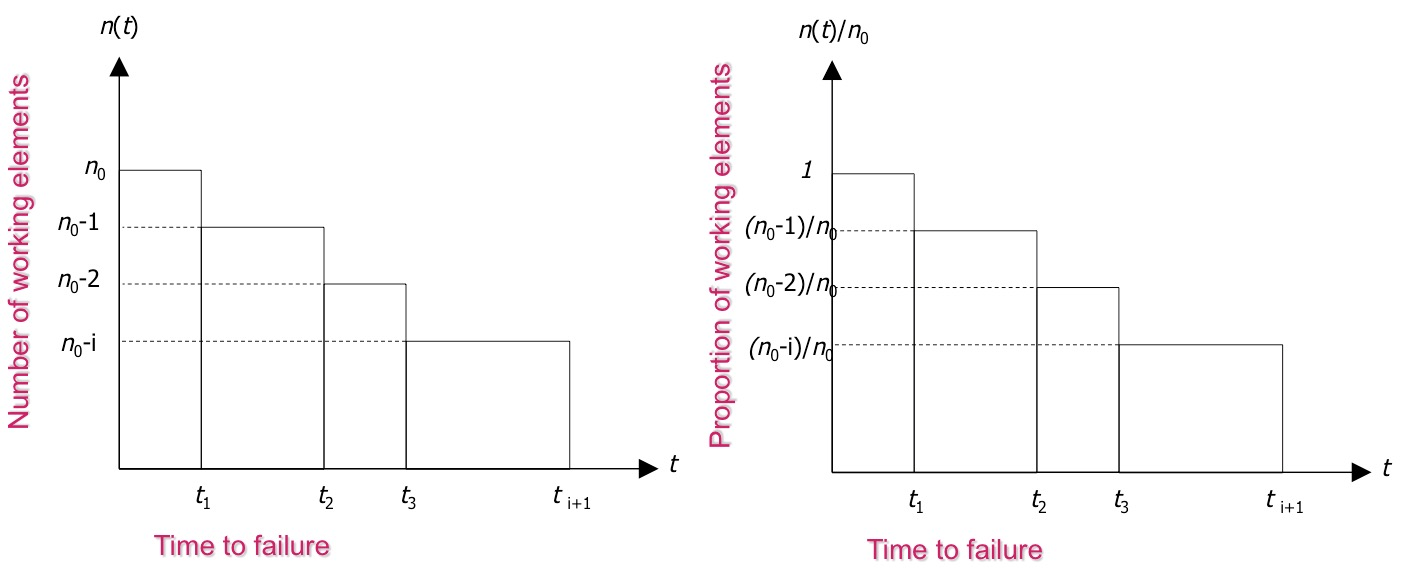
\includegraphics[width=\textwidth]{img/reliability-and-availability-2.png}
\end{figure}

\noindent
The function:
\begin{equation}
    \dfrac{n\left(t\right)}{n_{0}}
\end{equation}
Is the \definition{empirical function of reliability} that, as $n_{0} \rightarrow \infty$, \textbf{converges to the value}: 
\begin{equation}
    \dfrac{n\left(t\right)}{n_0} \rightarrow R\left(t\right)
\end{equation}

\highspace
\begin{flushleft}
    \textcolor{Green3}{\faIcon{question-circle} \textbf{Ok, but what do we do with the reliability probability?}}
\end{flushleft}
Well, the exploitation of the reliability probability information is \textbf{used to compute}, for a complex system, its reliability in time and the \textbf{expected lifetime}. Note that the computation of the overall reliability starts from the component one.

\newpage

\begin{flushleft}
    \textcolor{Red2}{\faIcon{bookmark} \textbf{Reliability terminology}}
\end{flushleft}
The \textbf{Constant Failure rate of the reliability} is:
\begin{equation}
    \begin{array}{rcl}
        R\left(t\right) &=& e^{-\lambda \: t} \\ [.5em]
        \texttt{MTTF} &=& \displaystyle\int_{0}^{\infty} R\left(t\right) \:\mathrm{d}t = \dfrac{1}{\lambda}
    \end{array}
\end{equation}
\begin{figure}[!htp]
    \centering
    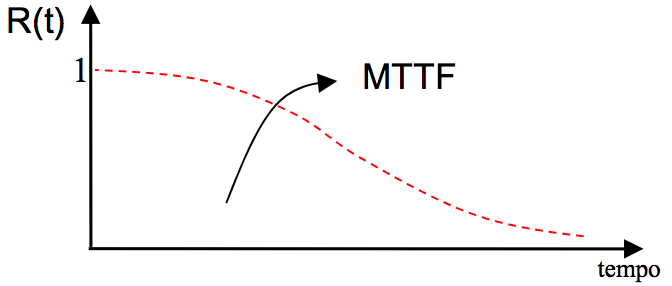
\includegraphics[width=.5\textwidth]{img/reliability-and-availability-4.png}
\end{figure}

\noindent
Then, to refer to it, we use the correct terminology.
\begin{itemize}
    \item The \underline{\textbf{Fault}} is a \textbf{defect within the system}.
    \item The \underline{\textbf{Error}} is a \textbf{deviation from the required operation of the system} or subsystem.
    \item \underline{\textbf{Failure}} is when the \textbf{system fails to perform its required function}.
\end{itemize}
\begin{figure}[!htp]
    \centering
    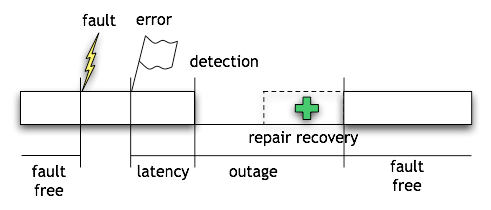
\includegraphics[width=.8\textwidth]{img/reliability-and-availability-3.png}
\end{figure}

\begin{examplebox}
    A flying drone with an automatic radar-guided landing system. An example of:
    \begin{itemize}
        \item Fault: the electromagnetic disturbances interfere with a radar measurement.
        \item Error: the radar-guided landing system calculates a wrong trajectory.
        \item Failure: the drone crashes to the ground.
    \end{itemize}
\end{examplebox}

\begin{examplebox}[: not always the fault-error-failure chain closes]
    A tele-surgery system. An example of:
    \begin{itemize}
        \item Fault: the radioactive ions change some memory cells' value (bitflip).
        \item Error: some frames of the video stream are corrupted.
        \item Failure: the surgeon kills the patient.
    \end{itemize}
    However, not always the fault-error-failure chain closes:
    \begin{itemize}
        \item Fault: the radioactive ions make some memory cells change value (bitflip), but the corrupted memory does not involve the video stream.
        \item Error: no frames are corrupted.
        \item Failure: the surgeon carries out the procedure.
    \end{itemize}
    As we can see, there is no activated fault! With the same logic, a flying drone with automatic radar-guided landing:
    \begin{itemize}
        \item Fault: electromagnetic disturbances interfere with a radar measurement.
        \item Error: the radar-guided landing system calculates a wrong trajectory, but then, based on subsequent correct radar measurements, it can recover the right trajectory.
        \item Failure: the drone safely lands.
    \end{itemize}
    Here, there is no propagated (or absorbed error).
\end{examplebox}

    \subsection{Disk performance}

\subsubsection{HDD}

We can calculate some performance metrics related to the types of delay of HDD (page \pageref{four types of hdd delay}).
\begin{itemize}
    \item \definition{Full Rotation Delay} $R$ is:
    \begin{equation}
        R = \dfrac{1}{\texttt{DiskRPM}}
    \end{equation}
    And in seconds:
    \begin{equation}
        R_{\text{sec}} = 60 \times R
    \end{equation}
    From the $R_{\text{sec}}$ we can also calculate the \definition{total rotation average}:
    \begin{equation}
        T_{\text{rotation AVG}} = \dfrac{R_{\text{sec}}}{2}
    \end{equation}

    \item \definition{Seek Time}, the \textbf{time to move the head to a different track}, which is divided into several phases:
    \begin{itemize}
        \item Acceleration
        \item Coasting (constant speed)
        \item Deceleration
        \item Settling
    \end{itemize}
    The $T_{\text{seek}}$ modelling considers a linear dependency with the distance. Also, the \definition{seek average} is:
    \begin{equation}
        T_{\text{seek AVG}} = \dfrac{T_{\text{seek MAX}}}{3}
    \end{equation}

    \item \definition{Transfer time}. It is the \textbf{time that data is either read from or written to the surface}. It \textbf{includes} the time the \textbf{head needs to pass on the sectors} and the \textbf{I/O transfer}. The \definition{Controller Overhead} is the \textbf{buffer management} (data transfer) and \textbf{interrupt sending time}.

    Transfer time and Controller Overhead are together because they are required to calculate some interesting metrics.
    \begin{itemize}
        \item \definition{Service Time} $T_{\text{I/O}}$
        \begin{equation}
            T_{\text{I/O}} = T_{\text{seek}} + T_{\text{rotation}} + T_{\text{transfer}} + T_{\text{overhead}}
        \end{equation}

        \item \definition{Response Time}
        \begin{equation}
            T_{\text{queue}} + T_{\text{I/O}}
        \end{equation}
        Where $T_{\text{queue}}$ depends on queue-length, resource utilization, mean and variance of disk service time and request arrival distribution.
    \end{itemize}
    \newpage
    \begin{figure}[!htp]
        \centering
        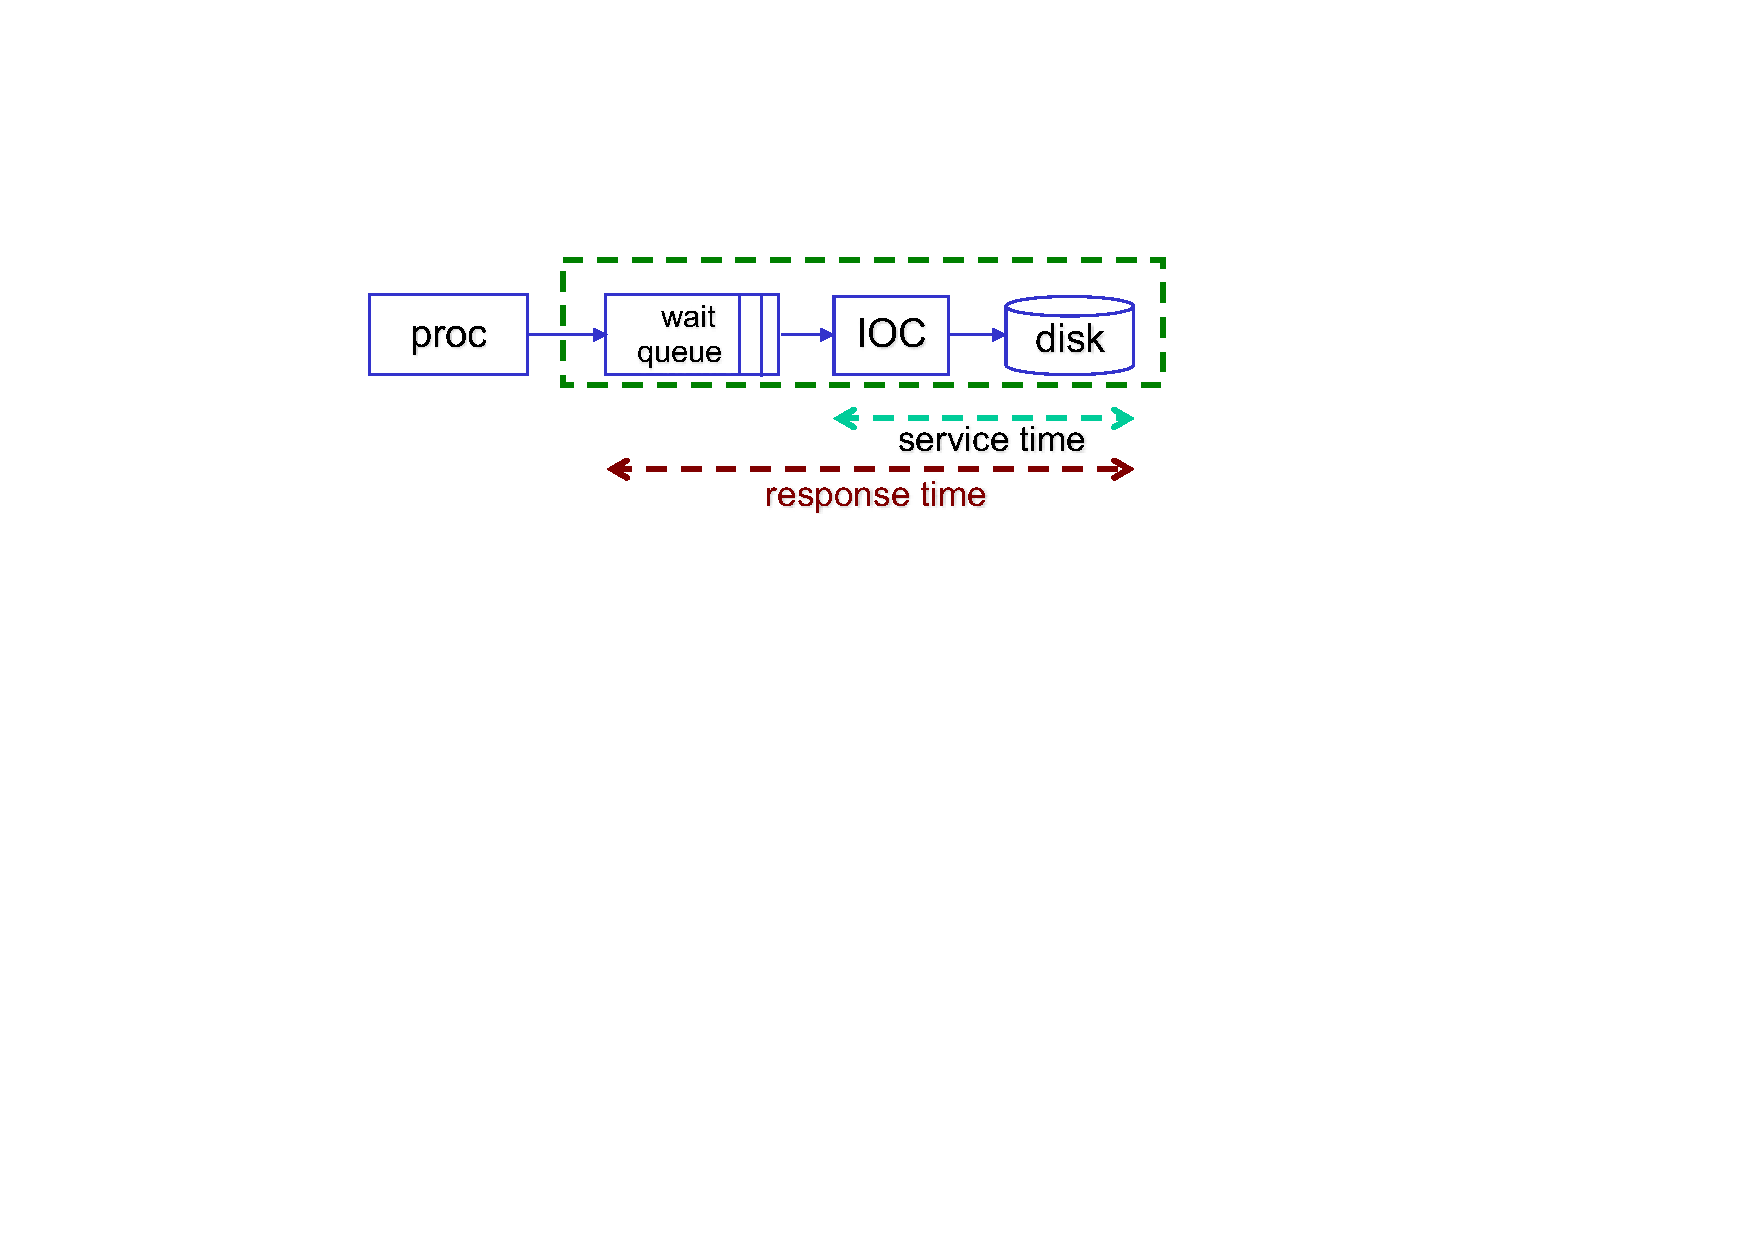
\includegraphics[width=.7\textwidth]{img/performance-hdd-1.pdf}
        \caption{Service and response time.}
    \end{figure}
\end{itemize}
    \subsection{Scalability and performance of datanceters}

    %%%%%%%%%%%%%%%%%%%%%%%%%%
    % Bibliography and index %
    %%%%%%%%%%%%%%%%%%%%%%%%%%
    \pagestyle{fancy}
\fancyhead{} % clear all header fields
\fancyhead[R]{\nouppercase{\leftmark}}

\bibliography{bibtex}{}
\bibliographystyle{plain}

\newpage

\printindex
\end{document}